\documentclass[12pt,a4paper]{article}

% ============================================================
% PACOTES
% ============================================================
\usepackage[utf8]{inputenc}
\usepackage[T1]{fontenc}
\usepackage[brazilian]{babel}
\usepackage{amsmath,amssymb}
\usepackage{graphicx}
\usepackage{booktabs}
\usepackage{caption}
\usepackage{float}
\usepackage{geometry}
\usepackage{hyperref}
\usepackage{xcolor}
\usepackage{enumitem}
\usepackage{array}
\usepackage{longtable}

\geometry{margin=2.5cm}
\hypersetup{
    colorlinks=true,
    linkcolor=blue,
    citecolor=blue,
    urlcolor=blue
}

% ============================================================
% CABEÇALHO / TÍTULO
% ============================================================
\title{
    \Large \textbf{Avanços em Inteligência Artificial} \\
    \large EELT7025 --- PPGEE, UFPR \\[0.3cm]
    \normalsize Exercícios da Aula 04 \\
    \normalsize Aprendizado Não-Supervisionado (\emph{Clustering})
}
\author{Adriely Teixeira de Paula, Betina Zynger Capaverde, Emilio Gaudeda Junior}
\date{\today}

% ============================================================
\begin{document}

\maketitle
\tableofcontents
\newpage

% ============================================================
\section*{Dataset utilizado}
\addcontentsline{toc}{section}{Dataset utilizado}

Os dois exercícios percorrem, sobre \textbf{um único dataset real de sinais de máquina rotativa}, o roteiro completo de \emph{clustering}: extração de atributos $\rightarrow$ EDA $\rightarrow$ pré-processamento $\rightarrow$ particionamento/hierárquico/densidade (\textbf{Exercício 1}) $\rightarrow$ modelos probabilísticos/grafos $\rightarrow$ algoritmos avançados $\rightarrow$ métricas internas e externas $\rightarrow$ síntese comparativa (\textbf{Exercício 2}).

\textbf{Dataset:} \emph{SCIG-3phase-Dataset}, do repositório \href{https://github.com/InnovaPower/MitDev-Eletrica}{InnovaPower/MitDev-Eletrica}, commit \texttt{b091742}, DOI \texttt{10.5281/zenodo.17161986}. Referência: Tominaga \emph{et al.}, \emph{A condition monitoring dataset based on electrical signals for a squirrel cage induction generator}, \textbf{Data in Brief} 63 (2025) 112286. Licença CC-BY-4.0.

\textbf{Bancada:} gerador de indução de gaiola de esquilo (SCIG) acionado acima da velocidade síncrona e conectado à rede por conversor com \textbf{controle orientado por campo}. As faltas são inseridas por um contator que permanece fechado por \textbf{400\,ms}, de $t = 1{,}0$\,s a $t = 1{,}4$\,s, com resistência de falta de \textbf{2,6\,$\Omega$}. Todos os sinais são amostrados a \textbf{20\,kHz} em registros de \textbf{3\,s}, com \textbf{35 canais} por ensaio.

\textbf{Conjunto completo utilizado --- 225 ensaios:}
\begin{itemize}[nosep]
    \item \textbf{108} ensaios \texttt{FAULT\_TURNS} --- curto \textbf{entre espiras}, 12 pares de derivação $\times$ 9 pontos de operação.
    \item \textbf{108} ensaios \texttt{FAULT\_WINDINGS} --- curto \textbf{entre enrolamentos}, 12 pares $\times$ 9 pontos de operação.
    \item \textbf{9} ensaios \texttt{HEALTHY}, cobrindo as nove combinações de velocidade (1200/1500/1800\,rpm) e torque (5,2/6,4/8,0\,N$\cdot$m).
\end{itemize}

\textbf{Rótulos reais.} O dataset traz rótulos verdadeiros, de modo que o item 12 é atendido sem recorrer a pseudo-rótulo. Foram usados dois:
\begin{enumerate}[nosep]
    \item \textbf{Condição} --- saudável $\times$ falta entre espiras $\times$ falta entre enrolamentos (3 classes).
    \item \textbf{Regime de operação} --- nove níveis de velocidade $\times$ torque.
\end{enumerate}

\textbf{Desenho cruzado.} Como existem faltas dos dois tipos em \emph{todos} os nove pontos de operação, os dois rótulos são \textbf{cruzados}: nenhuma conclusão sobre condição fica confundida com ponto de operação.

\textbf{Limitação assumida, verificada na fonte.} Todos os 225 ensaios usam \texttt{R026}, isto é, \textbf{resistência de falta fixa em 2,6\,$\Omega$}. A severidade varia apenas pelo par de derivação, ou seja, pelo número de espiras curto-circuitadas. Logo \textbf{severidade e posição no enrolamento são confundidas por construção da bancada} e não podem ser separadas com estes dados.

\newpage
% ============================================================
\section*{A investigação: como este relatório chegou às suas conclusões}
\addcontentsline{toc}{section}{A investigação: como este relatório chegou às suas conclusões}

Este trabalho \textbf{inverteu a própria conclusão} no meio do caminho. Como o percurso é parte do resultado --- e porque os dois erros cometidos são do tipo que qualquer análise de diagnóstico pode cometer --- ele está registrado aqui antes dos itens do enunciado.

\subsubsection*{Ato 1 --- O primeiro laudo dizia que não dava}

A análise inicial pegou as \textbf{três correntes de fase}, segmentou em janelas de 50\,ms e extraiu estatísticas temporais e harmônicos ímpares. Os doze algoritmos formaram grupos excelentes --- que separavam o \textbf{ponto de operação} da máquina, não o seu estado de saúde. O ARI contra condição ficava entre $-0{,}10$ e $0{,}00$.

O laudo foi além e explicou: a malha de controle orientada por campo regula as correntes de estator e \emph{mascara} a assimetria antes que ela chegue aos terminais. Conclusão registrada na época: \emph{``não é limitação dos algoritmos, é propriedade física do sistema''}.

\subsubsection*{Ato 2 --- A pergunta que desmontou o laudo}

\emph{Foi descartado algum dado que poderia servir?}

Cada arquivo tem \textbf{35 canais}. Foram usados \textbf{três}. Nunca foram abertos: as tensões nos terminais, as correntes no referencial girante, o fluxo estimado, as tensões de comando do conversor e --- o ponto constrangedor --- \textbf{o esforço dos controladores PI}. O laudo afirmava que o controle mascarava a falta sem nunca ter olhado o que o controle estava fazendo.

\subsubsection*{Ato 3 --- A hipótese física, declarada antes de olhar o dado}

Um curto assimétrico decompõe-se em sequência positiva, negativa e zero. A sequência negativa gira no \textbf{sentido contrário} ao campo. Para um observador que acompanha o campo --- o referencial $dq$ --- algo que gira ao contrário na mesma velocidade passa \textbf{duas vezes por volta}.

Portanto: \textbf{a assimetria não desaparece; ela reaparece em $2\omega$ no referencial girante}. O estudo inicial mediu os harmônicos 3, 5 e 7 e nunca o segundo. A assinatura estava no arquivo o tempo inteiro, num lugar onde nenhum instrumento foi apontado.

\subsubsection*{Ato 4 --- Três provas antes de acreditar}

\begin{enumerate}[nosep]
    \item \textbf{Contra o acaso.} Dois modelos nulos independentes, com correção de Bonferroni para 79 atributos. Nove atributos passam nos dois.
    \item \textbf{Liga-desliga.} Se é a falta, o indicador sobe quando o contator fecha e \textbf{volta} quando ele abre --- deriva de ensaio sobe e fica. Subiu $+2{,}68\sigma$ e voltou a $-0{,}03\sigma$.
    \item \textbf{Dose-resposta.} Quanto maior a corrente de falta, maior o indicador: $\rho = 0{,}738$, $p = 8{,}8\times10^{-20}$. \textbf{O indicador não apenas acende --- ele mede.}
\end{enumerate}

\subsubsection*{Ato 5 --- O segundo erro: 9\% dos dados}

Ao declarar que certas limitações eram insolúveis, veio a segunda pergunta incômoda: \emph{o dataset completo foi baixado?}

A pasta de trabalho tinha \textbf{21 dos 225 ensaios}. Faltavam as faltas nos outros oito pontos de operação e \textbf{um segundo tipo de falta inteiro} --- entre enrolamentos. A ``limitação'' de que os rótulos não eram cruzados era artefato da amostra, não do dataset. Com o conjunto completo o desenho passou a ser \textbf{perfeitamente cruzado}.

\subsubsection*{Ato 6 --- O desfecho}

Com 5715 janelas, nove regimes e três condições, a assinatura em $2f$ funciona nos \textbf{nove} pontos de operação: \textbf{84\%} de detecção nas faltas entre enrolamentos, \textbf{56\%} entre espiras, com 6 alarmes falsos em 531 janelas saudáveis.

E o fecho: o \textbf{ruído} do DBSCAN --- as janelas que o algoritmo não consegue encaixar em lugar nenhum --- deixou de ser um regime de operação inocente e passou a ser \textbf{90,4\% falta}. HDBSCAN e OPTICS chegam a 100\%. \textbf{O que o algoritmo chamava de lixo virou o diagnóstico.}

\subsubsection*{A moral, que é o resultado central}

Não foi um algoritmo melhor que resolveu; foi \textbf{olhar no lugar certo}. O \emph{Spectral Clustering} passa de pior método ($\text{ARI} = -0{,}001$) a terceiro melhor ($0{,}516$) \textbf{sem que uma linha de sua configuração mude}. Só mudou o que ele recebe de entrada.

\begin{quote}
\noindent O sistema não esconde a falta. Ele a \textbf{muda de lugar}: da amplitude das correntes de fase para a ondulação em $2\omega$ das grandezas do referencial girante, inclusive do esforço que o controlador gasta corrigindo o problema. Quem mede apenas estatística temporal de $I_a$, $I_b$ e $I_c$ não vê nada. Quem demodula em $2\theta$ vê.
\end{quote}

\newpage
% ============================================================
% EXERCÍCIO 1
% ============================================================
\section{Exercício 1: Extração de Atributos, EDA e \emph{Clustering} por Partição, Hierarquia e Densidade}

\noindent\emph{Este exercício é o Ato 2 da investigação: a auditoria dos canais, a construção dos atributos que faltavam e os três primeiros algoritmos. O item 6 é onde a conclusão começa a virar.}

\subsection{Seleção de canais: o que entra e o que fica de fora}

Antes de extrair qualquer atributo, os 35 canais de cada ensaio foram auditados. Usar apenas as três correntes de fase, como é hábito em MCSA, é uma decisão que precisa ser justificada --- e aqui ela \textbf{não se sustenta}.

\begin{table}[H]
\centering
\caption{Auditoria dos 35 canais}
\begin{tabular}{lll}
\toprule
Constatação & Canais & Decisão \\
\midrule
Constantes & \texttt{Flux\_ref}, \texttt{Idref} & Descartados: informação nula \\
Definem o rótulo regime & \texttt{Spd} ($r = 1{,}000$ com velocidade) & Descartados: usá-los \\
                        & \texttt{Torq\_mec} ($r = 1{,}000$ com torque) & seria circular \\
                        & \texttt{Torq\_ele} ($r = 0{,}988$) & \\
Definem o rótulo condição & \texttt{Ifault}, \texttt{Fault\_relay} & Só como controle positivo \\
Referências redundantes & \texttt{Va\_ref} $\equiv$ \texttt{Da}, e análogos & Mantida a grandeza medida \\
Referência de fase & \texttt{Theta\_est} & Usado na demodulação, não como atributo \\
\bottomrule
\end{tabular}
\end{table}

\noindent Restam \textbf{dois blocos}, separados pela observabilidade real em campo:
\begin{itemize}[nosep]
    \item \textbf{Terminal elétrico}: $I_a, I_b, I_c, V_a, V_b, V_c, V_{cc}$ --- o que um monitor nos terminais enxerga.
    \item \textbf{Interno do conversor}: $I_d, I_q, V_d, V_q$, tensões de comando, ações dos controladores PI e fluxo estimado --- o que o firmware do acionamento enxerga.
\end{itemize}

\textbf{Correção metodológica registrada.} A primeira tentativa de medir redundância correlacionou as formas de onda CA cruas e produziu o absurdo $I_a \equiv V_b$. Correlação de Pearson entre senoides de mesma frequência mede o \textbf{cosseno da diferença de fase}, não informação compartilhada. A redundância passou a ser medida sobre \textbf{atributos de janela}, que é o espaço onde o agrupamento de fato opera.

\subsection{Item 1 --- Segmentação em janelas e extração de atributos}

\subsubsection*{Comprimento da janela}

A frequência elétrica foi \textbf{medida}, não suposta: a FFT da corrente de fase em regime permanente dá \textbf{40,0\,Hz} a 1200\,rpm, e o ângulo elétrico \texttt{Theta\_est} gira a 39,6\,Hz. Logo \textbf{50\,ms correspondem a exatamente 2 ciclos elétricos completos}. O comprimento foi varrido (25, 50, 100, 200 e 300\,ms) contra modelo nulo: a janela de 50\,ms é a única em que o \emph{k-means} converge para solução única entre 40 inicializações distintas.

\subsubsection*{Sobreposição: zero}

Janelas sobrepostas compartilham amostras e portanto \textbf{não são independentes}. Isso infla o $n$ aparente, estreita artificialmente qualquer intervalo de confiança e invalida os modelos nulos por permutação usados na validação. Com 5715 janelas o $n$ não é o gargalo, de modo que a sobreposição não traria benefício que compensasse o custo estatístico.

\subsubsection*{Os 79 atributos}

\begin{table}[H]
\centering
\caption{Composição do vetor de atributos}
\begin{tabular}{llc}
\toprule
Família & Conteúdo & $n$ \\
\midrule
Estatística temporal & RMS, curtose, assimetria e \emph{crest factor} de $I_a, I_b, I_c, V_a, V_b, V_c$ & 24 \\
Engenharia fasorial  & Impedância por fase e desequilíbrio; ângulo de fator de & 26 \\
                     & potência; componentes simétricas de tensão e corrente; & \\
                     & harmônicos 3, 5, 7; energia nas bandas 1--5 e 5--9,9\,kHz & \\
Referencial $dq$     & Nível, dispersão e \textbf{ondulação em $2f$} de nove canais internos & 27 \\
Barramento CC        & Nível e dispersão de $V_{cc}$ & 2 \\
\midrule
\textbf{Total}       & & \textbf{79} \\
\bottomrule
\end{tabular}
\end{table}

Os harmônicos são estimados por \textbf{demodulação coerente},
\[
A_{p,k} \;=\; 2\,\bigl|\,\overline{x_p\,e^{-jk\theta}}\,\bigr|,
\]
usando o ângulo elétrico medido. O método é exato mesmo com frequência variando e \textbf{não sofre do limite de resolução de \emph{bin}} da FFT --- o que importa aqui, pois a 50\,ms uma FFT teria resolução de 20\,Hz para harmônicos espaçados de 40\,Hz.

\textbf{Dois atributos merecem destaque porque não existiam na abordagem convencional.} A \textbf{impedância aparente por fase} $Z_p = A_1(V_p)/A_1(I_p)$ só é calculável porque as tensões entraram. E a \textbf{ondulação em $2f$},
\[
\text{ond2f}(x) \;=\; \bigl|\,2\,\overline{(x-\bar{x})\,e^{-j2\theta}}\,\bigr|,
\]
que mede a componente em $2\omega$ das grandezas no referencial girante. A motivação é física e anterior ao dado: \textbf{um curto assimétrico gera sequência negativa, e sequência negativa aparece em $2\omega$ no referencial que gira a $+\omega$.}

\begin{figure}[H]
    \centering
    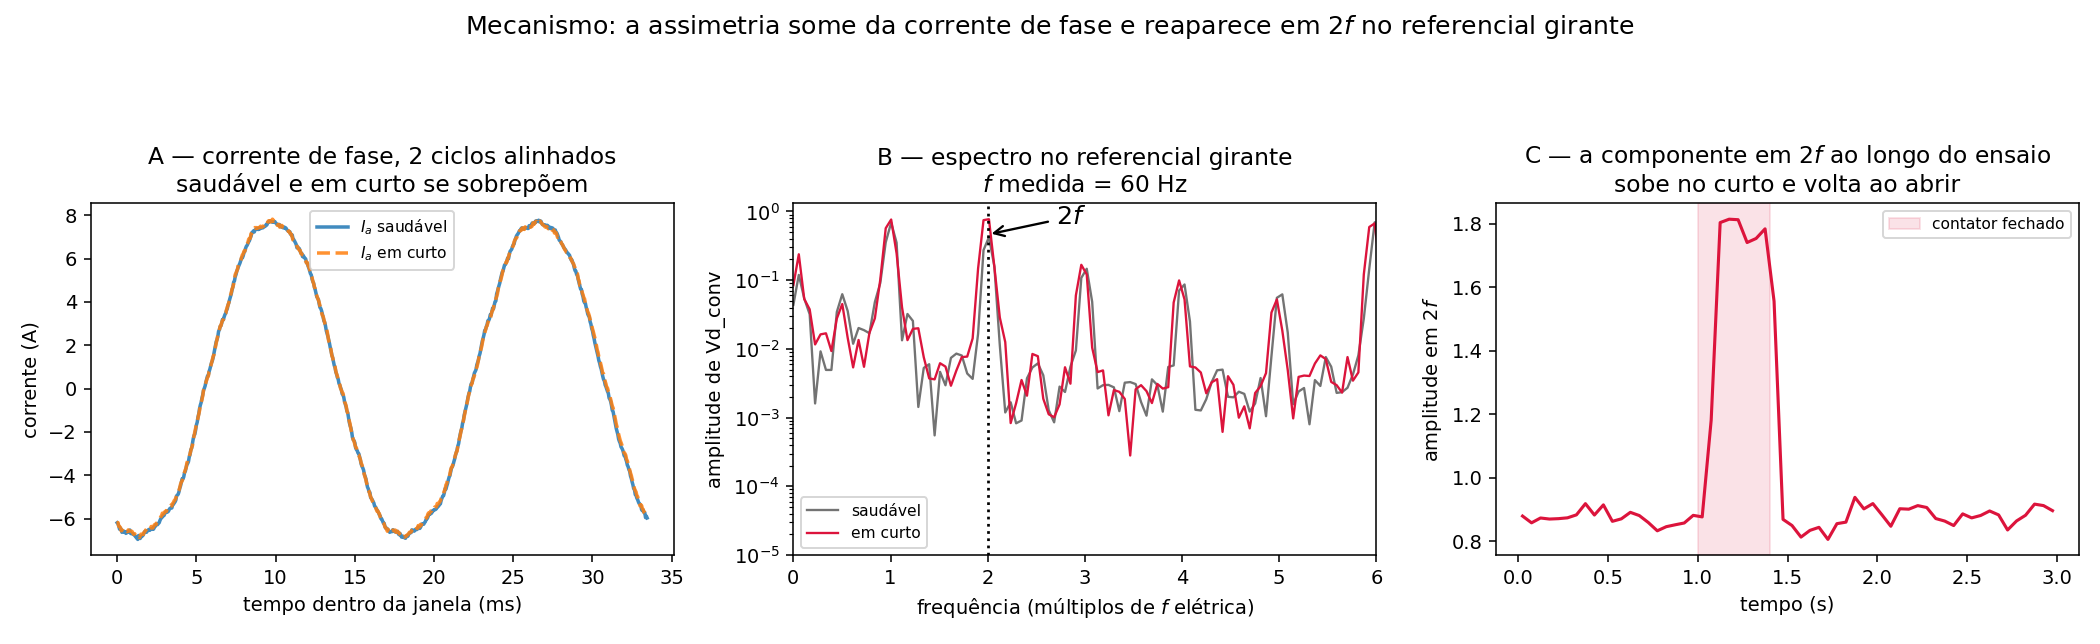
\includegraphics[width=\textwidth]{Figuras_Aula4/fig15-mecanismo-sequencia-negativa.png}
    \caption{O mecanismo em um único ensaio (\texttt{FAULT\_TURNS\_D17\_D20\_R026\_S1800\_T64}). \textbf{A}: a corrente de fase em dois ciclos alinhados pelo ângulo elétrico --- a janela saudável e a janela em curto se sobrepõem, e é por isso que o estudo inicial não viu nada. \textbf{B}: o espectro de uma grandeza do referencial girante nas mesmas duas janelas, com o eixo em múltiplos da frequência elétrica medida (59,6\,Hz) --- o pico em $2f$ sobe. \textbf{C}: a amplitude em $2f$ ao longo dos 3\,s, que sobe 1,9$\times$ quando o contator fecha e retorna exatamente à linha de base quando ele abre.}
    \label{fig:fig15}
\end{figure}

\noindent A Figura~\ref{fig:fig15} é a justificativa visual do trabalho inteiro: \textbf{os mesmos dados, o mesmo instante, a mesma máquina --- e a informação está num painel e não no outro}.

\subsubsection*{Verificação do contrato de dados}

\begin{table}[H]
\centering
\caption{Composição do conjunto de janelas: desenho perfeitamente cruzado}
\begin{tabular}{lccc}
\toprule
Regime & Falta entre enrolamentos & Falta entre espiras & Saudáveis \\
\midrule
S1200\_T5.2 / T6.4 / T8.0 & 72 cada & 72 cada & 491 cada \\
S1500\_T5.2 / T6.4 / T8.0 & 72 cada & 72 cada & 491 cada \\
S1800\_T5.2 / T6.4 / T8.0 & 72 cada & 72 cada & 491 cada \\
\midrule
\textbf{Total} & \textbf{648} & \textbf{648} & \textbf{4419} \\
\bottomrule
\end{tabular}
\end{table}

\noindent \textbf{5715 janelas}, \textbf{79 atributos}, \textbf{zero} valores ausentes e \textbf{zero} valores não finitos. A cronologia do relé foi conferida em todos os 216 ensaios com falta.

\subsection{Item 2 --- Análise exploratória}

\begin{figure}[H]
    \centering
    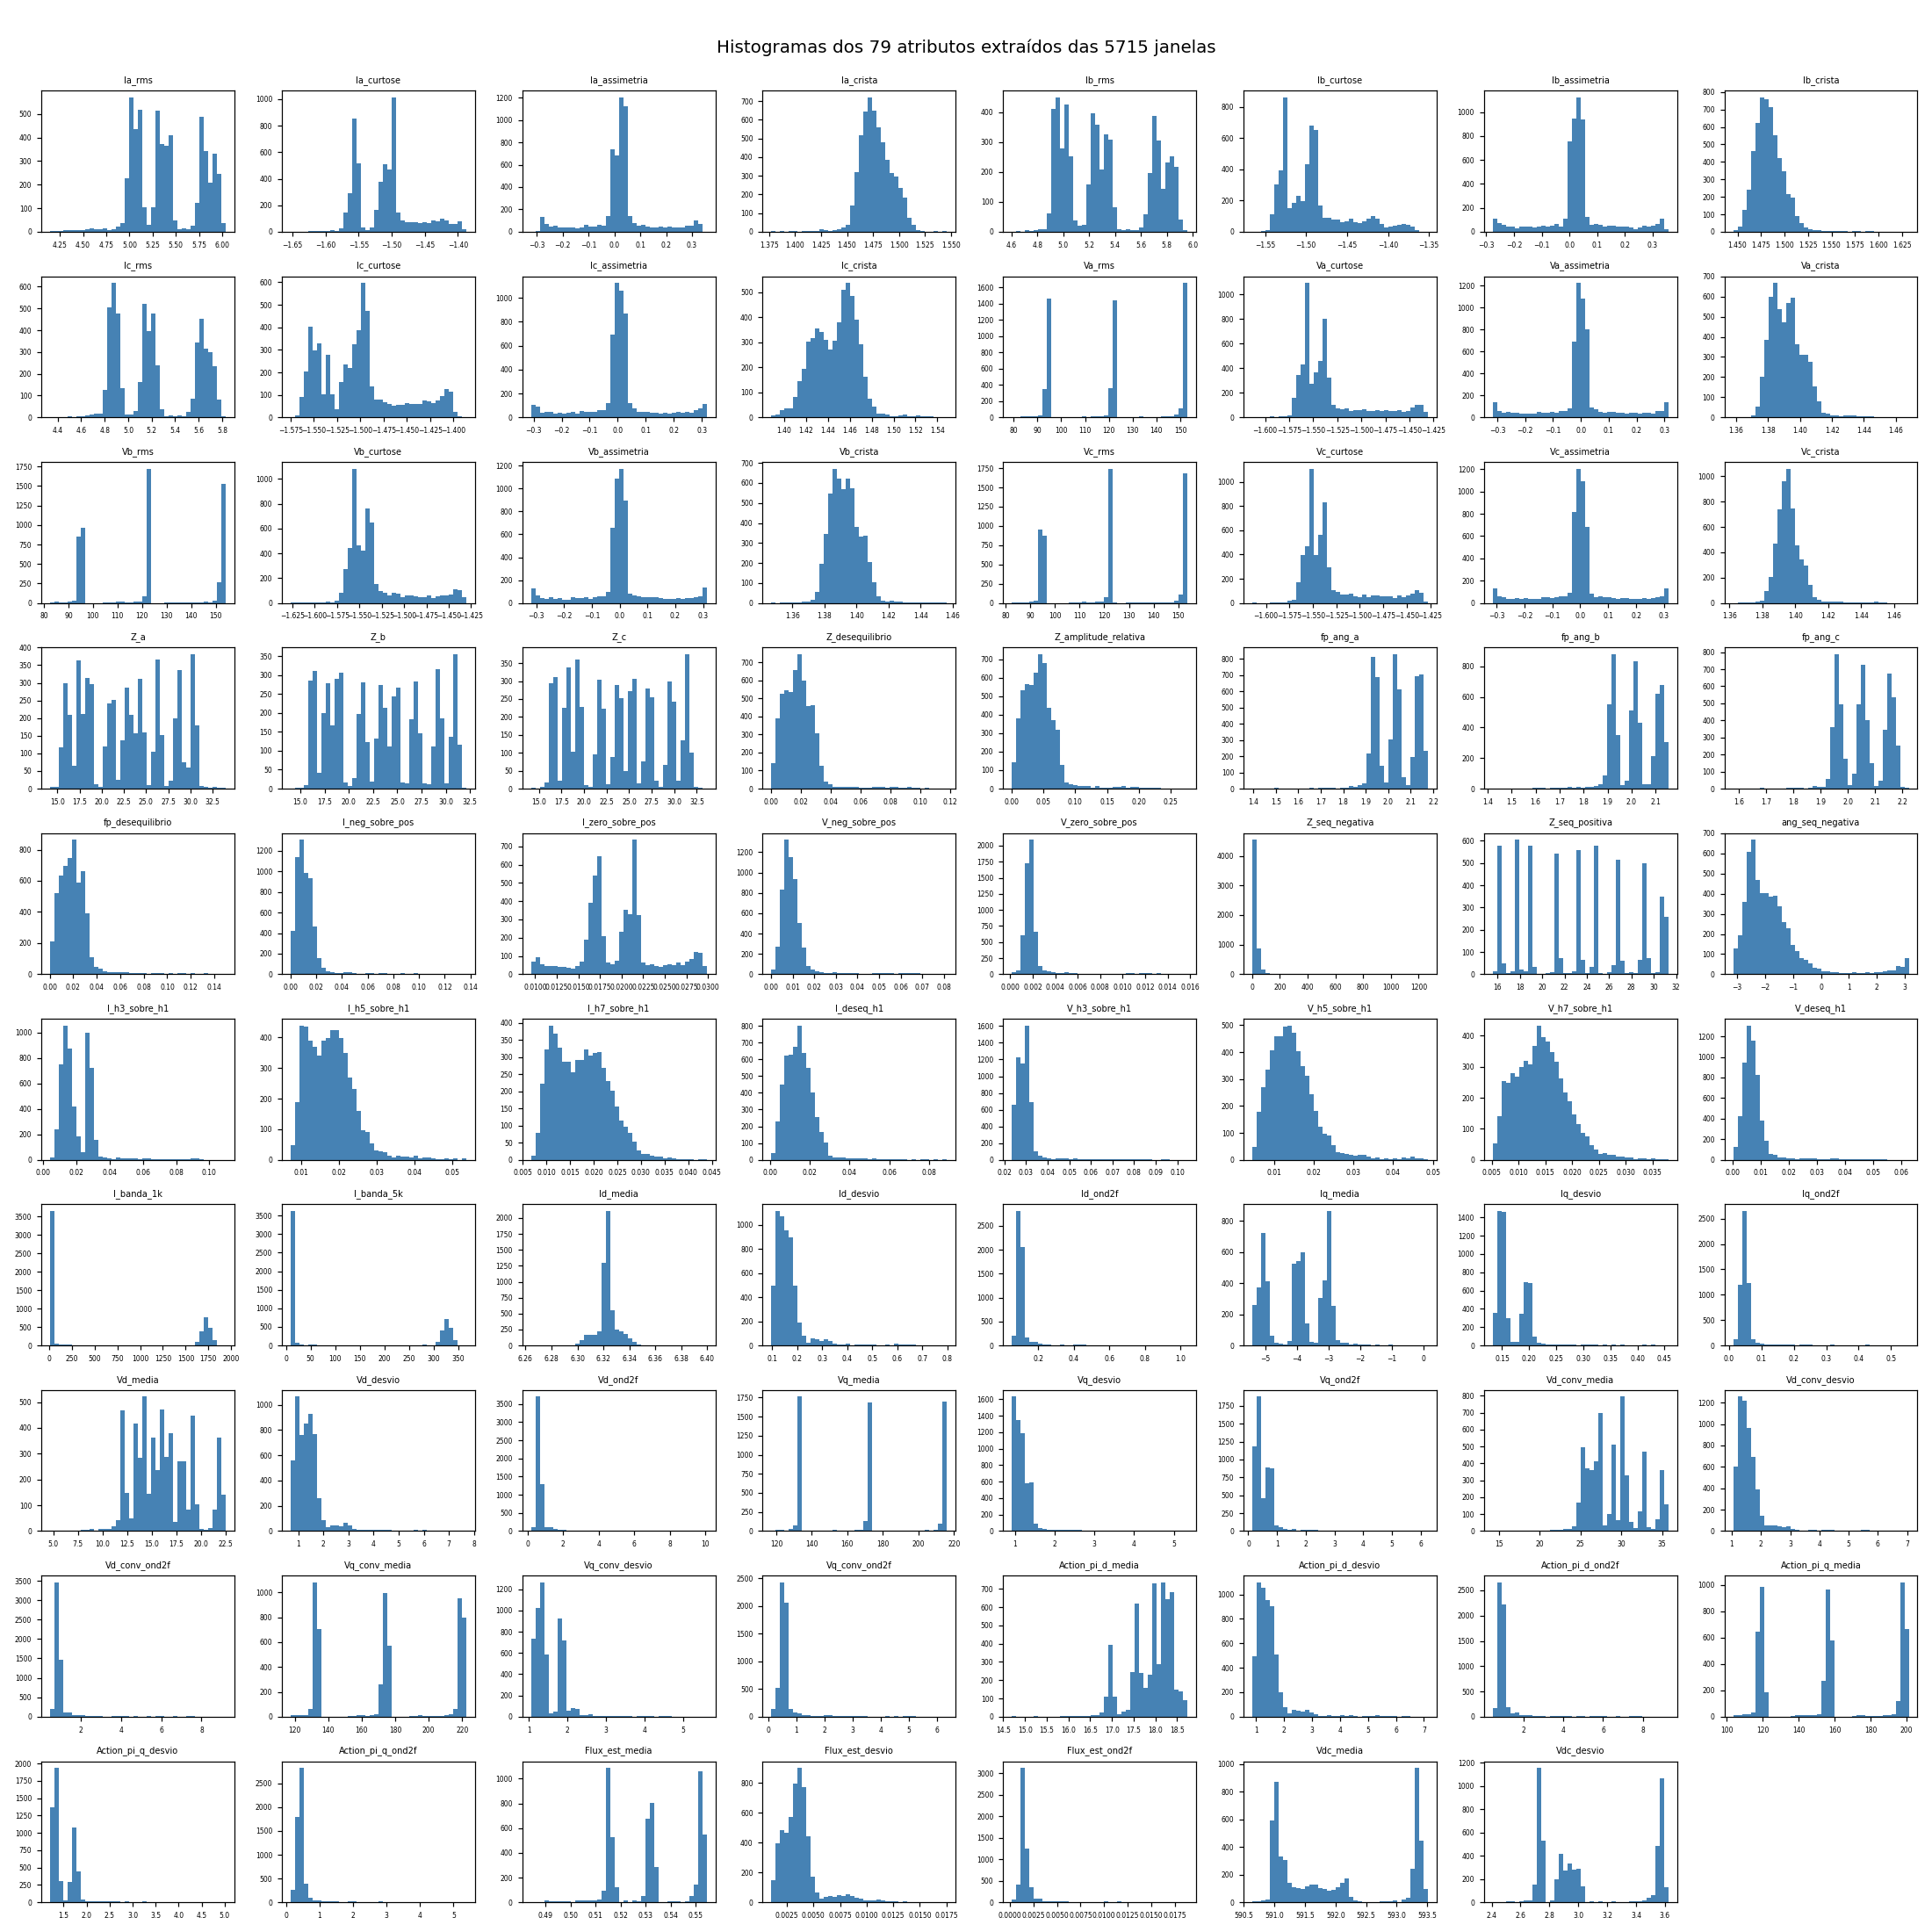
\includegraphics[width=\textwidth]{Figuras_Aula4/fig1-histogramas-atributos.png}
    \caption{Histogramas dos 79 atributos extraídos das 5715 janelas.}
    \label{fig:fig1}
\end{figure}

\begin{figure}[H]
    \centering
    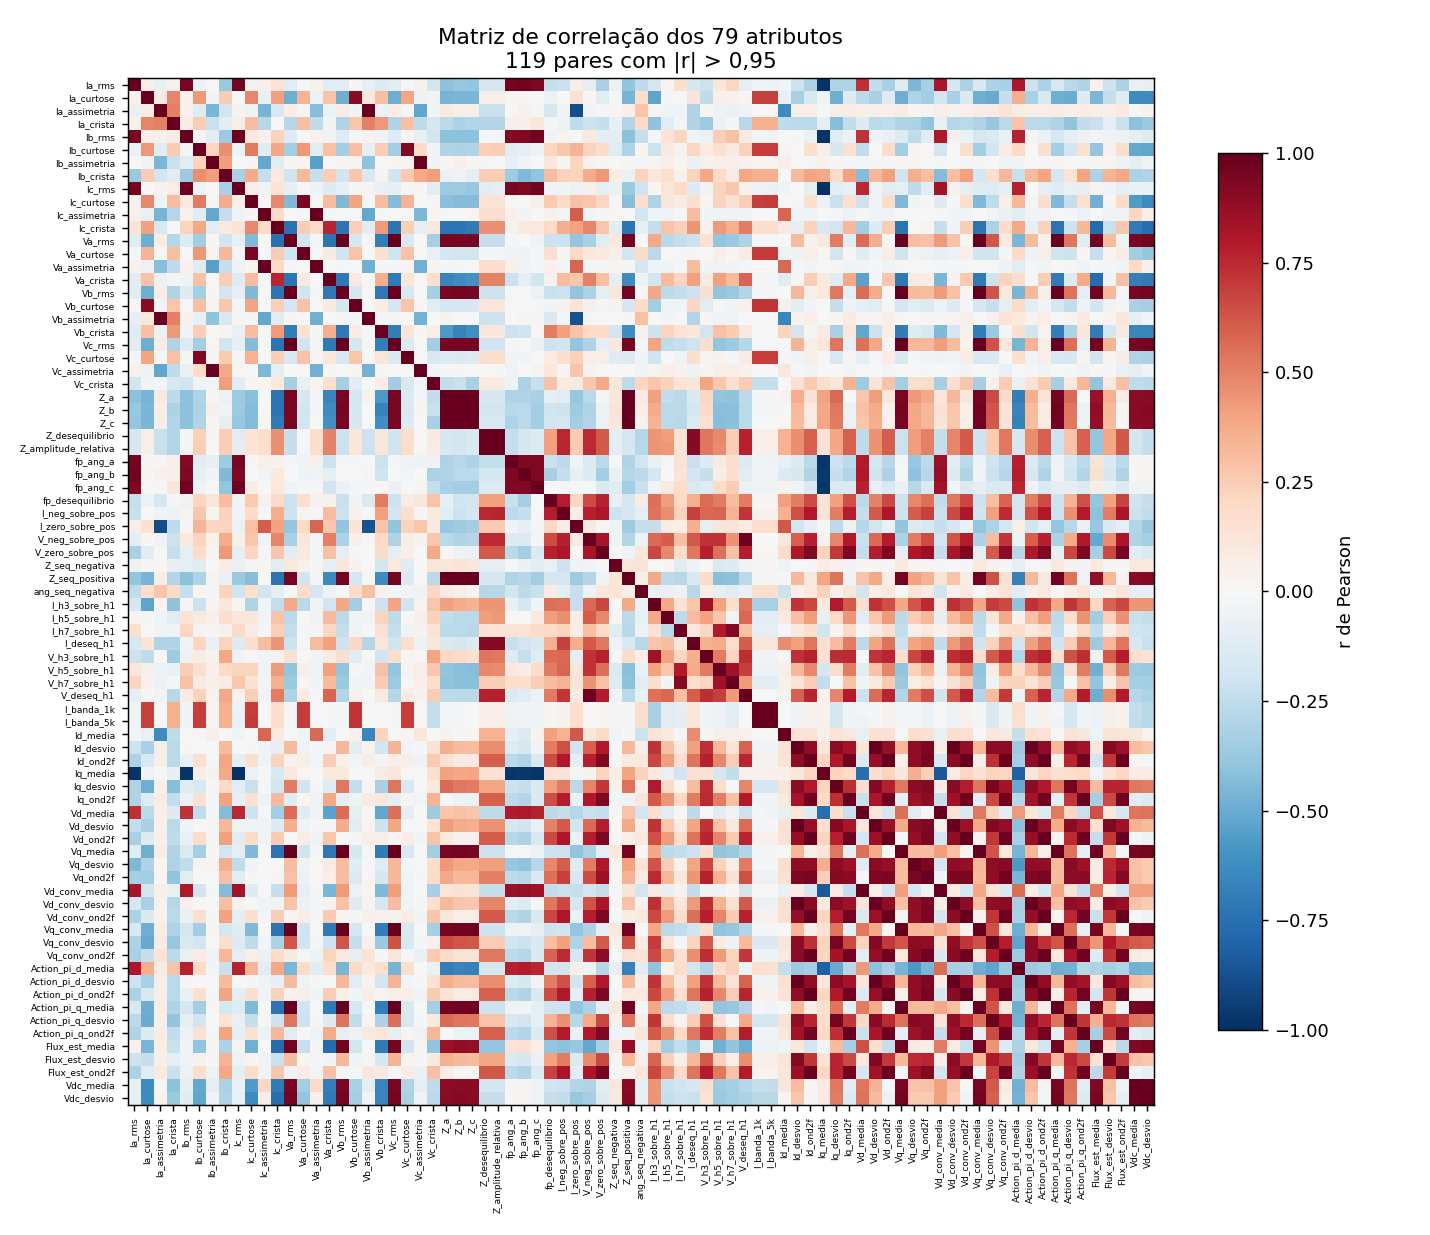
\includegraphics[width=0.82\textwidth]{Figuras_Aula4/fig2-matriz-correlacao.png}
    \caption{Matriz de correlação de Pearson entre os 79 atributos.}
    \label{fig:fig2}
\end{figure}

\noindent Há \textbf{119 pares} com $|r| > 0{,}95$. A redundância concentra-se entre grandezas que medem amplitude do mesmo sinal quase senoidal, e entre grandezas do referencial $dq$ que rastreiam o mesmo ponto de operação.

\begin{figure}[H]
    \centering
    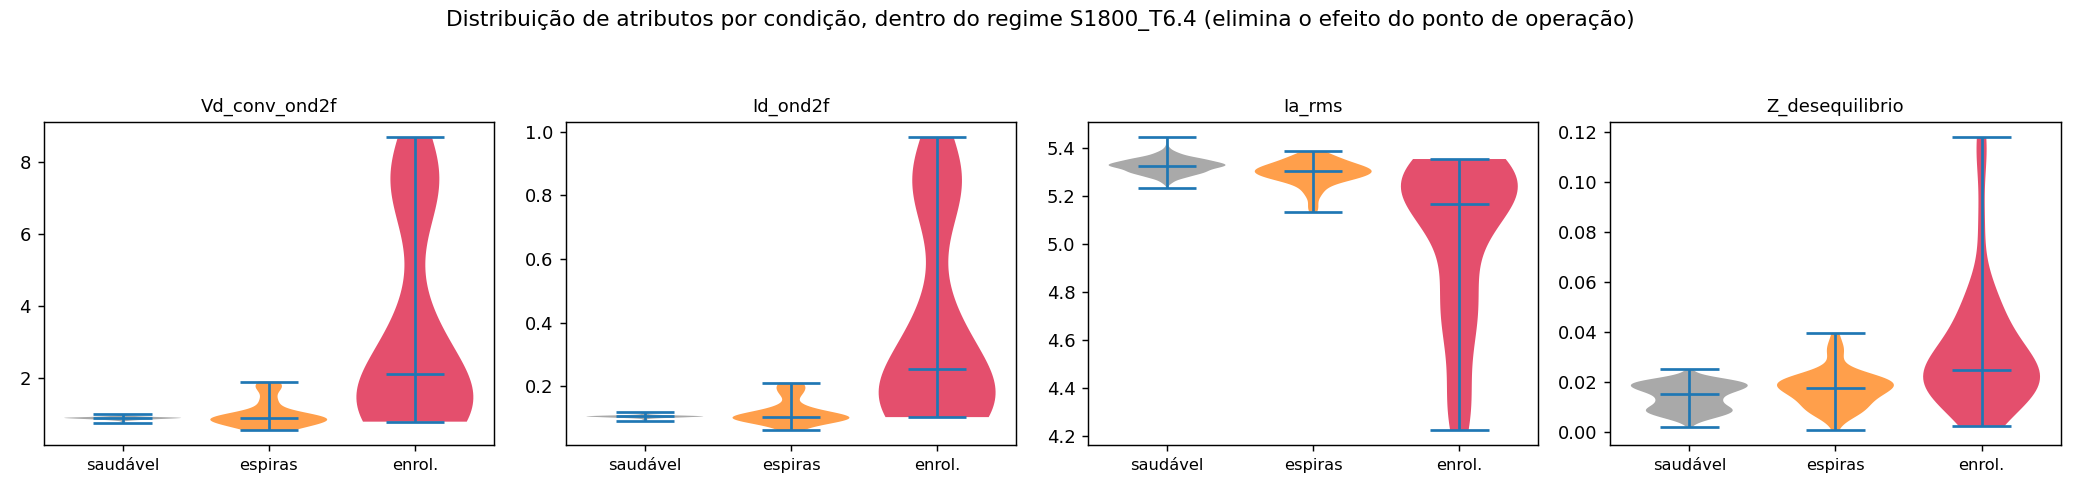
\includegraphics[width=\textwidth]{Figuras_Aula4/fig3-distribuicao-por-condicao.png}
    \caption{Distribuição de quatro atributos por condição, restrita ao regime S1800\_T6.4 para eliminar o efeito do ponto de operação.}
    \label{fig:fig3}
\end{figure}

\noindent O contraste é o ponto da figura. Em \texttt{Ia\_rms} e \texttt{Z\_desequilibrio} as três condições praticamente se sobrepõem. Em \texttt{Vd\_conv\_ond2f} e \texttt{Id\_ond2f} as faltas se deslocam. \textbf{O atributo certo separa; o atributo convencional, não.}

\subsection{Item 3 --- Normalização e redução de dimensionalidade}

\textbf{Critério do escalador, fixado antes de observar o resultado:} usar \texttt{RobustScaler} se a curtose mediana dos atributos exceder 3; caso contrário, \texttt{StandardScaler}. A curtose mediana medida foi \textbf{2,01}, abaixo do limiar, de modo que se adotou o \textbf{\texttt{StandardScaler}}.

Dois espaços de atributos são carregados em paralelo por todo o restante do trabalho:

\begin{itemize}[nosep]
    \item \textbf{Espaço A} --- os 79 atributos com escala global. É o pipeline convencional.
    \item \textbf{Espaço B} --- os 9 atributos de ondulação em $2f$, padronizados pelas janelas \emph{saudáveis do próprio regime}. A normalização por regime torna o indicador adimensional e comparável entre pontos de operação.
\end{itemize}

\begin{figure}[H]
    \centering
    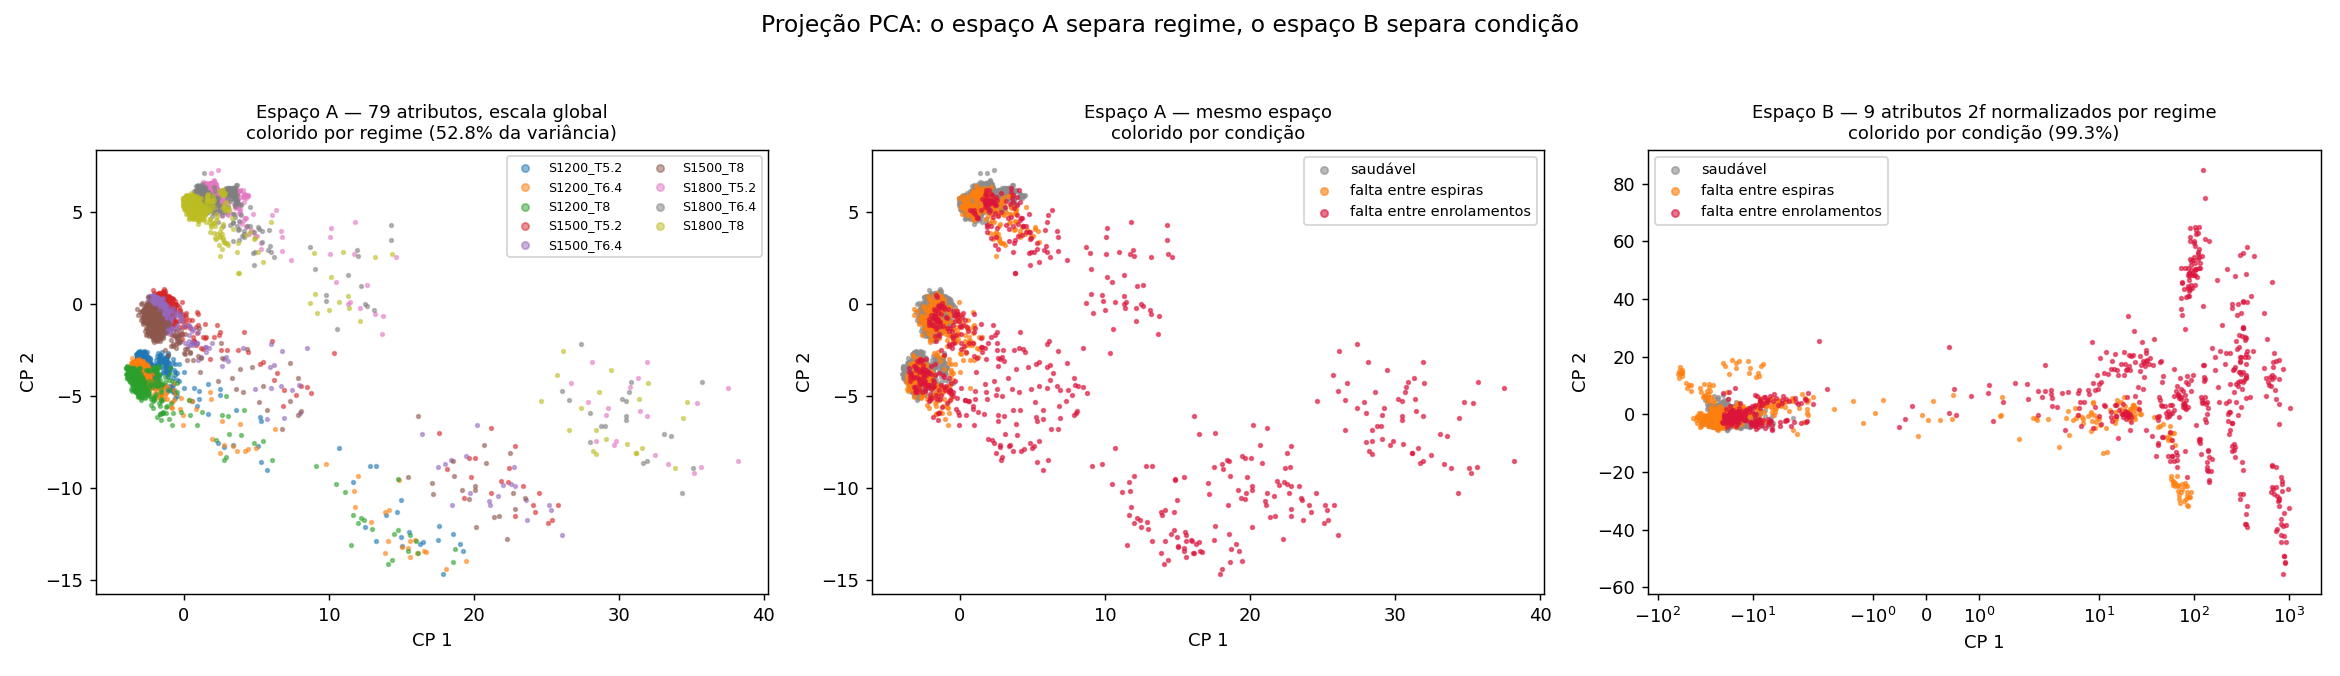
\includegraphics[width=\textwidth]{Figuras_Aula4/fig4-pca-regime-condicao.png}
    \caption{Projeção PCA dos dois espaços. O espaço A carrega a estrutura de regime; o espaço B carrega a estrutura de condição.}
    \label{fig:fig4}
\end{figure}

\noindent No espaço A duas componentes explicam \textbf{52,8\%} da variância e são necessárias \textbf{10} componentes para 90\%. No espaço B duas componentes explicam \textbf{99,3\%}: o sinal de falta é essencialmente \textbf{bidimensional}.

\subsection{Item 4 --- K-Means, escolha de $K$ e variante}

\begin{figure}[H]
    \centering
    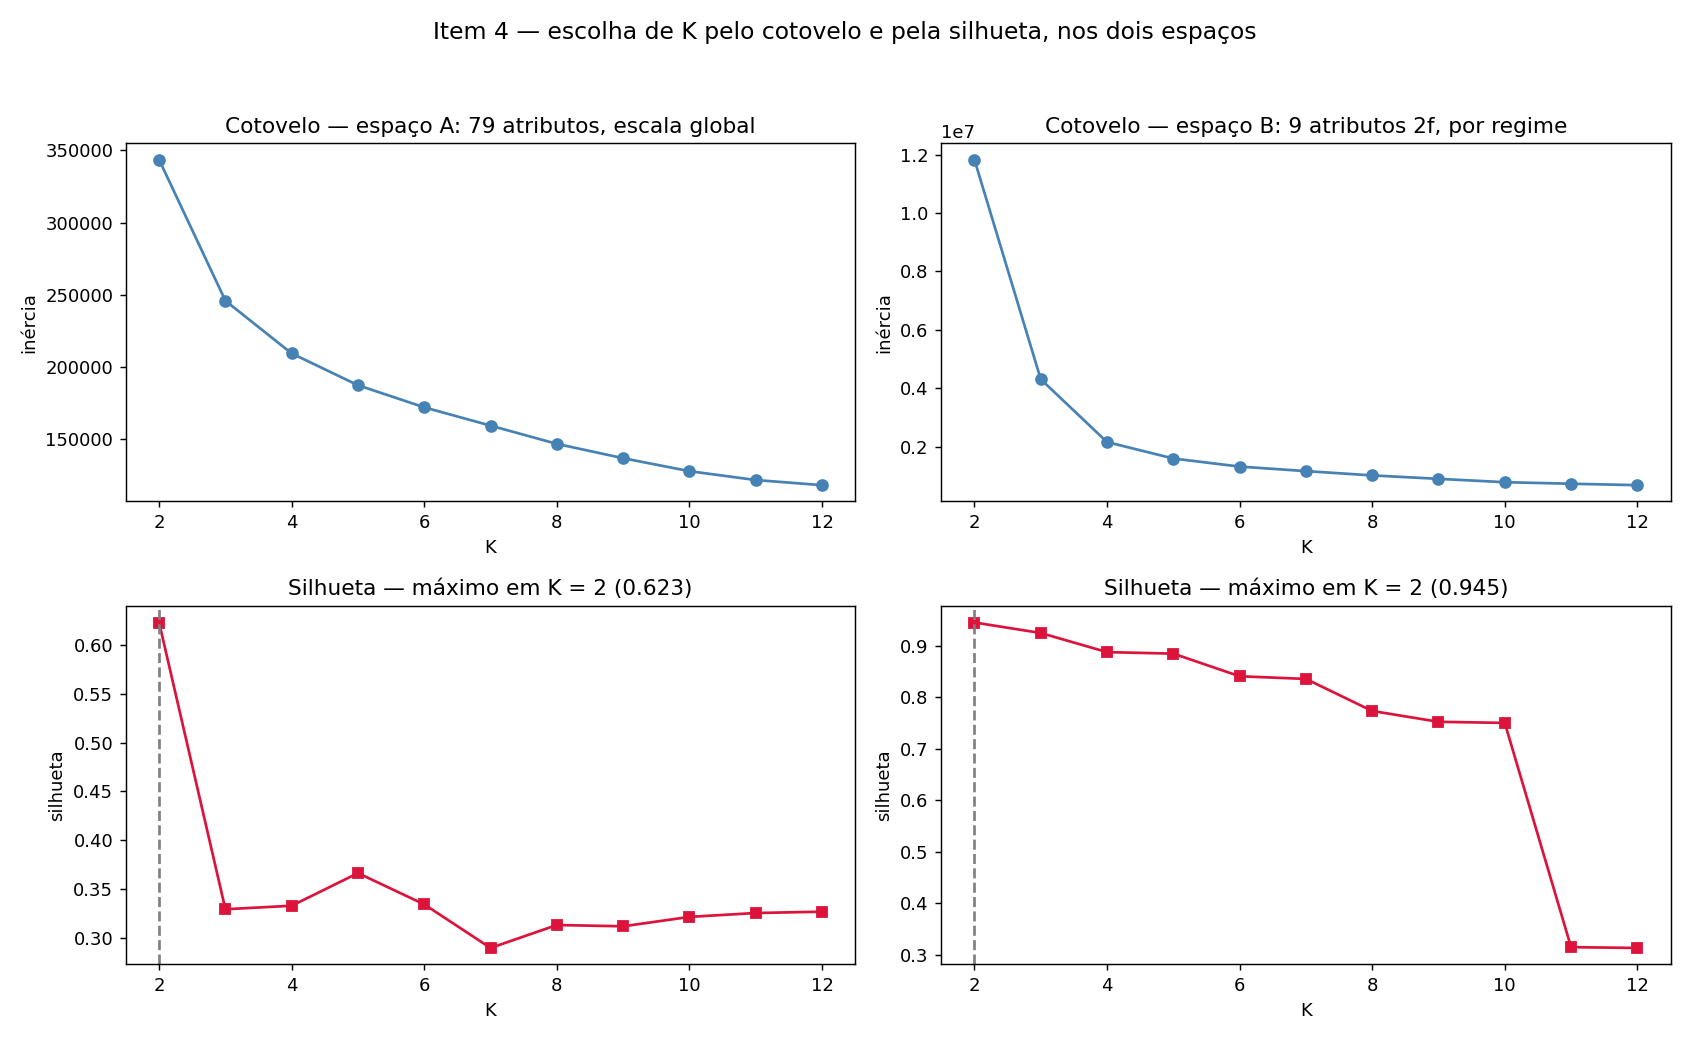
\includegraphics[width=\textwidth]{Figuras_Aula4/fig5-cotovelo-silhueta.png}
    \caption{Método do cotovelo e coeficiente de silhueta para $K$ de 2 a 12, nos dois espaços.}
    \label{fig:fig5}
\end{figure}

\noindent A silhueta aponta $\mathbf{K = 2}$ \textbf{nos dois espaços} --- 0,623 no espaço A e \textbf{0,945} no espaço B. Existem, porém, \textbf{três} classes reais.

\textbf{Essa tensão é informativa e não foi contornada.} Com 77,3\% de janelas saudáveis, o critério de silhueta prefere separar ``massa saudável'' de ``resto'' a dividir o resto em dois. É um efeito de \textbf{desbalanceamento}, não de falha do algoritmo. Nas tabelas dos itens 11 e 12 adota-se $K = 3$, o número de classes conhecidas, e esta discordância fica registrada.

O \textbf{MiniBatch K-Means} foi aplicado como variante. No espaço B ele coincide com o K-Means em $K=2$, mas em $K=3$ o supera com folga (ARI 0,489 contra 0,177) --- uma inversão que decorre da inicialização e que ilustra por que variantes merecem ser testadas em vez de assumidas inferiores.

\subsection{Item 5 --- \emph{Clustering} hierárquico aglomerativo}

\begin{figure}[H]
    \centering
    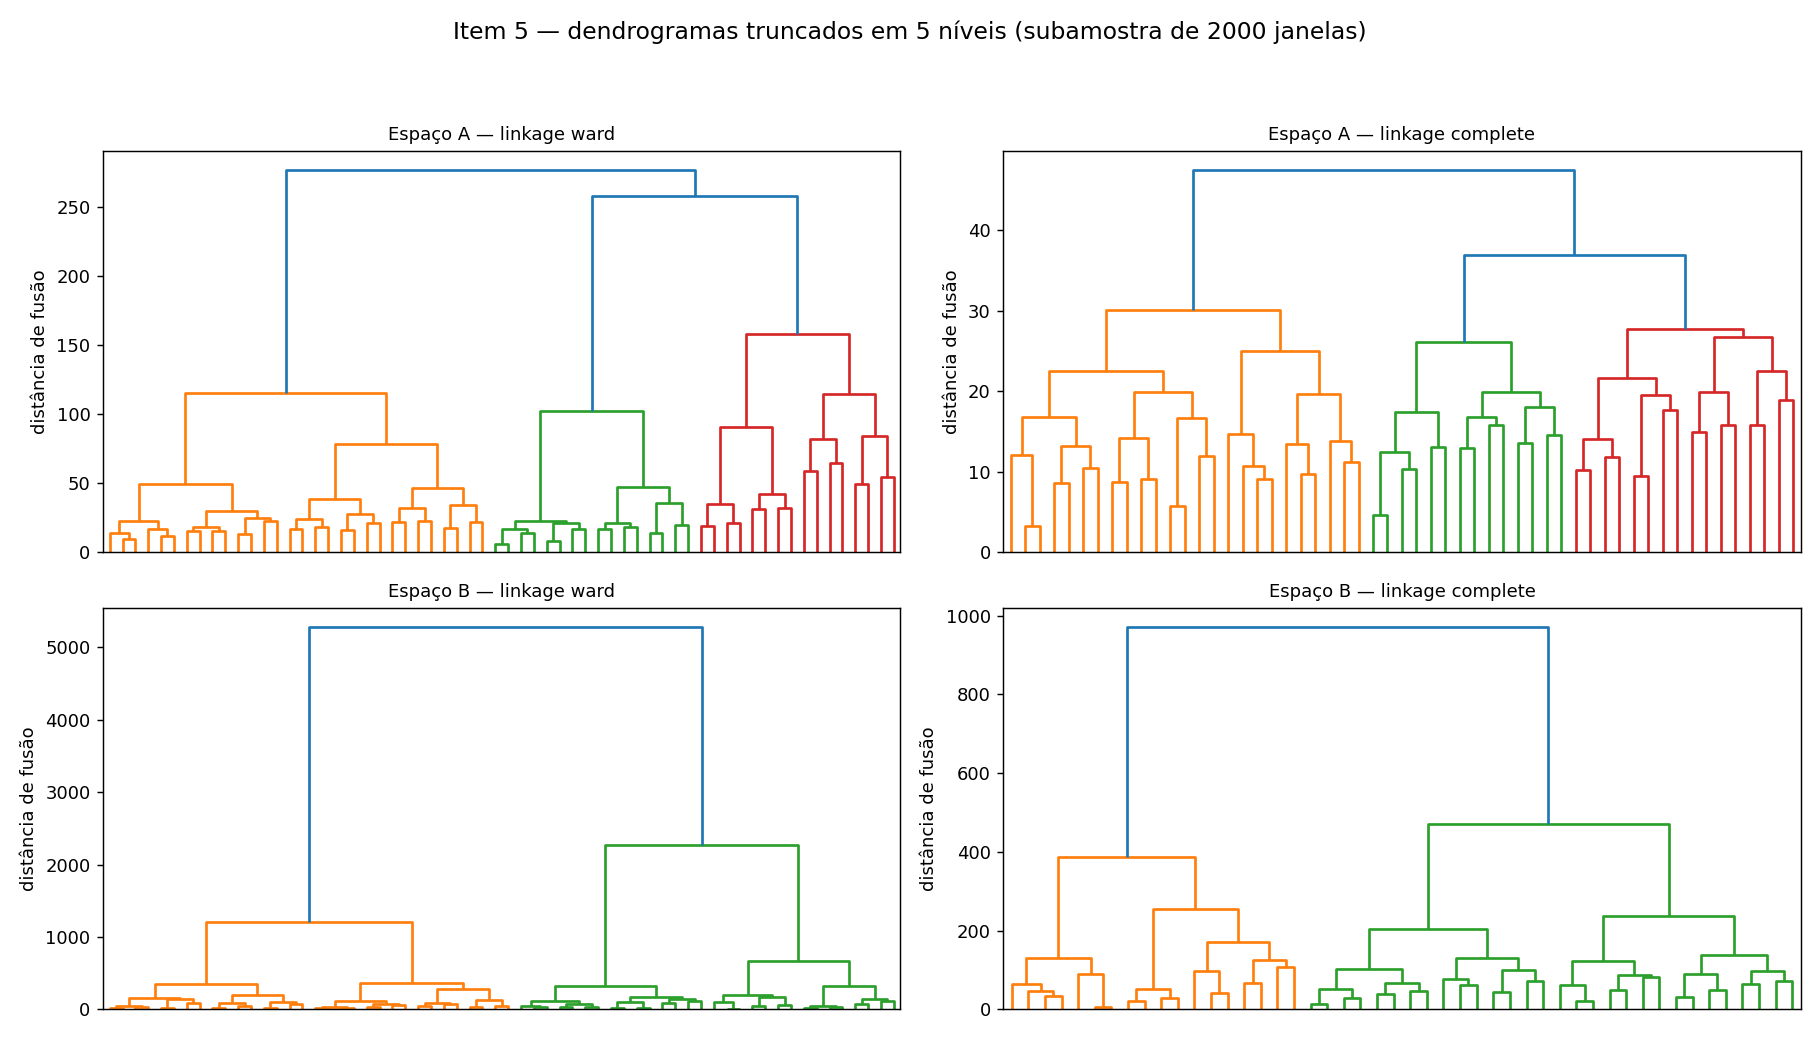
\includegraphics[width=\textwidth]{Figuras_Aula4/fig6-dendrogramas-ward-complete.png}
    \caption{Dendrogramas com \emph{linkage} Ward e Complete, nos dois espaços, truncados em cinco níveis sobre subamostra de 2000 janelas.}
    \label{fig:fig6}
\end{figure}

\noindent O \textbf{Ward} produz fusões equilibradas nos dois espaços. O \textbf{Complete} produz cadeias desbalanceadas, com um ramo absorvendo a maior parte das observações. Nenhum dos dois é competitivo para a tarefa de condição: no espaço B o Ward atinge ARI de 0,138 e o Complete 0,147, contra 0,592 do DBSCAN.

\subsection{Item 6 --- DBSCAN e interpretação do ruído}

\begin{figure}[H]
    \centering
    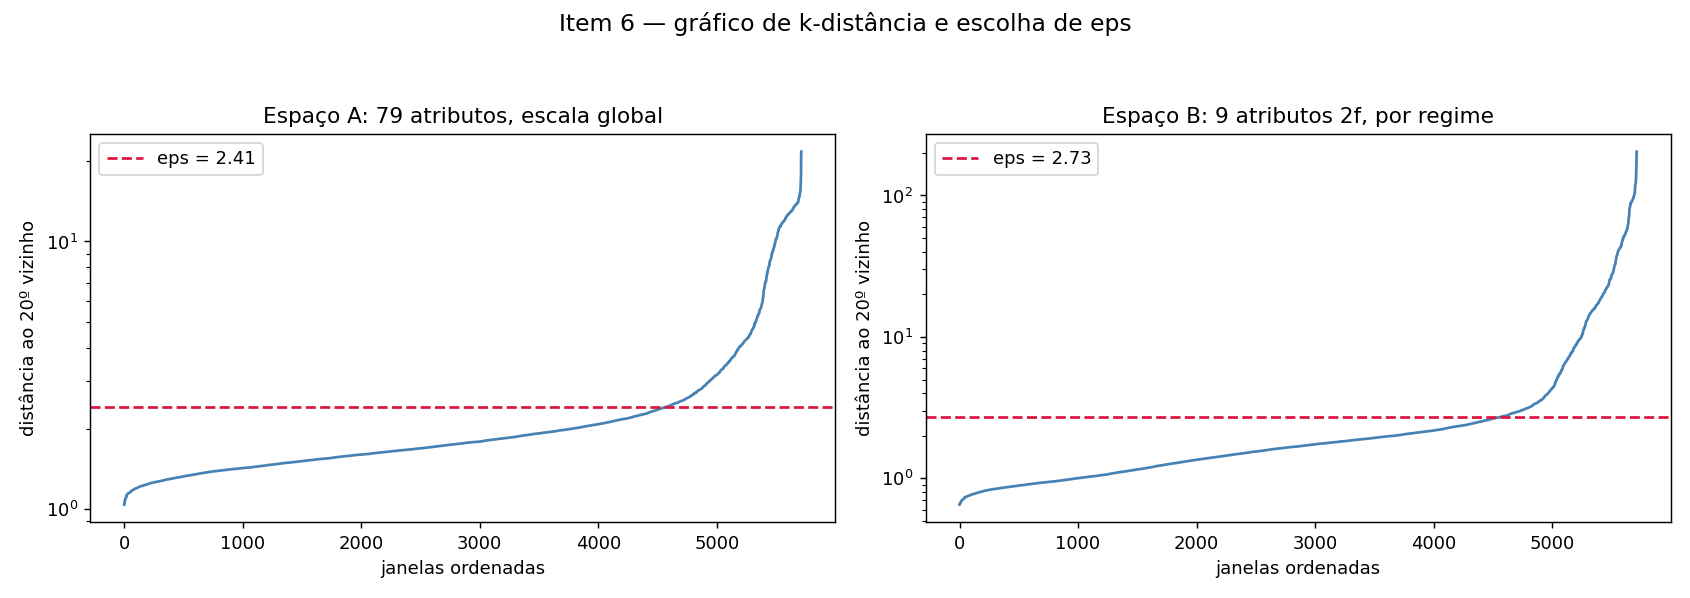
\includegraphics[width=\textwidth]{Figuras_Aula4/fig7-grafico-k-distancia.png}
    \caption{Gráfico de $k$-distância com $k=20$ e o \texttt{eps} escolhido, nos dois espaços. Escala vertical logarítmica.}
    \label{fig:fig7}
\end{figure}

\textbf{Correção de critério, registrada.} O joelho pela corda --- método usual --- \textbf{falha} neste conjunto. A curva de $k$-distância tem cauda muito longa: a razão entre o percentil 99 e a mediana é \textbf{49} no espaço B, contra 16 no espaço A. Isso é a assinatura de um núcleo muito denso com periferia muito esparsa, e o joelho geométrico devolve um \texttt{eps} grande demais, que funde tudo num grupo só. Adotou-se o \textbf{percentil 80 da curva}, verificado por varredura.

\begin{table}[H]
\centering
\caption{DBSCAN: composição do conjunto de ruído}
\label{tab:dbscan}
\begin{tabular}{lcccccc}
\toprule
Espaço & \texttt{eps} & Grupos & Ruído & Enrolamentos & Espiras & Saudáveis \\
\midrule
A & 2,41 & 11 & 723 (12,7\%) & 439 & 131 & 153 \\
B & 2,73 & 2  & 814 (14,2\%) & 488 & 248 & \textbf{78} \\
\bottomrule
\end{tabular}
\end{table}

\subsubsection*{Os pontos de ruído são anomalias reais ou apenas região de baixa densidade?}

\textbf{São anomalias reais.} No espaço B, \textbf{90,4\% das janelas de ruído são falta} --- 4,0 vezes a taxa base de 22,7\%. Apenas 78 das 4419 janelas saudáveis (1,8\%) caem no ruído.

Vale registrar que esta resposta \textbf{inverteu} em relação a uma análise preliminar feita apenas com as correntes de fase e um subconjunto de 21 ensaios. Naquele recorte o ruído era composto exatamente pelos três regimes S1500, com \textbf{zero} faltas, e a conclusão correta era ``baixa densidade, não anomalia''. Com o conjunto completo e o espaço de atributos certo, o ruído do DBSCAN passa a ser \textbf{o próprio alvo do diagnóstico}. A pergunta do enunciado, portanto, não tem resposta universal: ela depende do espaço de atributos, e só pode ser respondida medindo a composição do ruído.

\newpage
% ============================================================
% EXERCÍCIO 2
% ============================================================
\section{Exercício 2: Modelos Probabilísticos, Grafos, Algoritmos Avançados e Avaliação}

\noindent\emph{Este exercício é o Ato 6: nove algoritmos adicionais, as métricas e a síntese. O padrão que emerge é sempre o mesmo --- o algoritmo muda pouco, o espaço de atributos muda tudo.}

\subsection{Item 7 --- \emph{Gaussian Mixture Models} e seleção por BIC/AIC}

\begin{figure}[H]
    \centering
    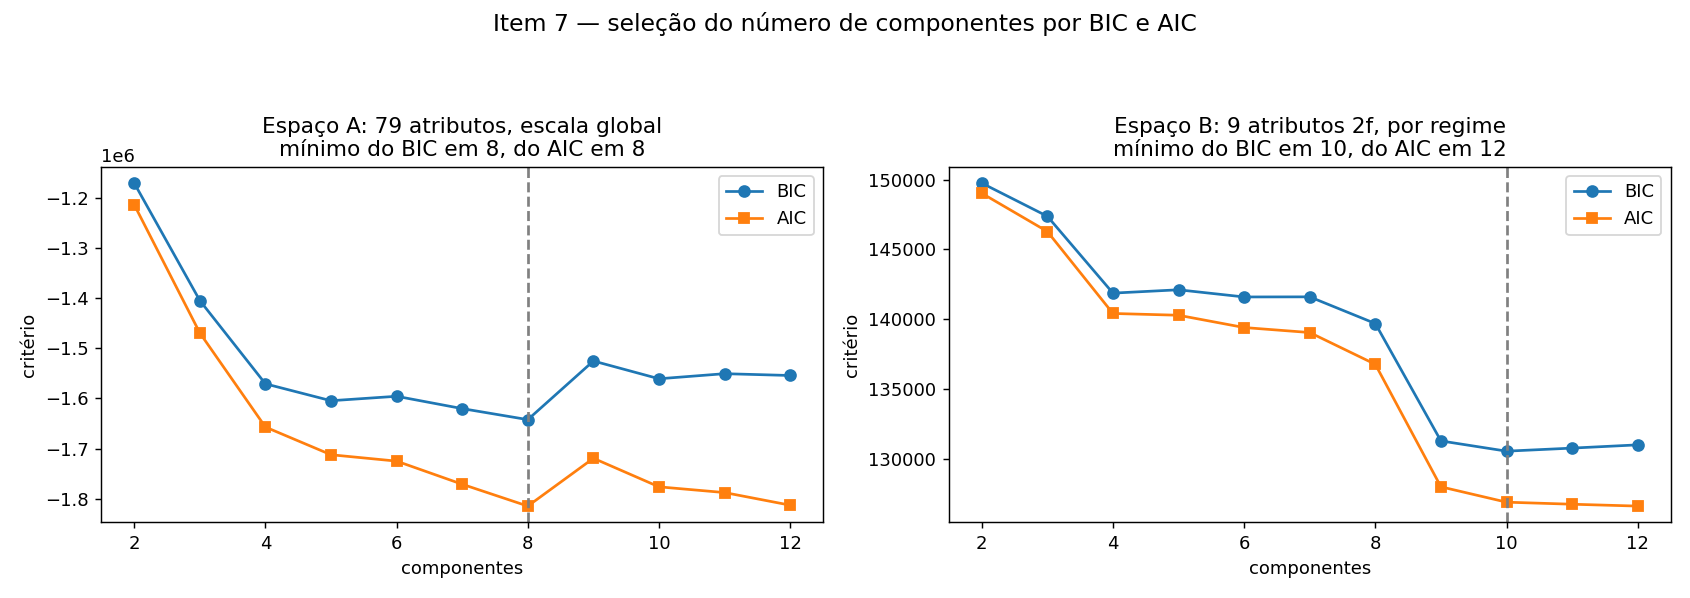
\includegraphics[width=\textwidth]{Figuras_Aula4/fig8-bic-aic-gmm.png}
    \caption{Critérios BIC e AIC para 2 a 12 componentes gaussianas, nos dois espaços.}
    \label{fig:fig8}
\end{figure}

\noindent No \textbf{espaço A} o BIC e o AIC concordam em \textbf{8} componentes --- próximo dos nove regimes, confirmando que este espaço codifica sobretudo o ponto de operação. No \textbf{espaço B} o BIC escolhe \textbf{10} e o AIC \textbf{12}, coerente com a penalização mais fraca da complexidade pelo AIC.

\textbf{Comparação \emph{soft} $\times$ \emph{hard}.} Aqui os dois espaços se comportam de maneira oposta, e isso é o achado do item:

\begin{itemize}[nosep]
    \item \textbf{Espaço A}: probabilidade máxima com mediana \textbf{1,0000} e \textbf{100,0\%} das janelas acima de 0,99. A atribuição suave \textbf{colapsa na rígida} e o GMM não agrega incerteza alguma.
    \item \textbf{Espaço B}: mediana 0,9945 e apenas \textbf{62,3\%} acima de 0,99. Aqui a atribuição probabilística \textbf{carrega incerteza real}, concentrada nas janelas de falta leve que ficam na fronteira.
\end{itemize}

\noindent A concordância com o K-Means confirma a leitura: ARI de 0,668 no espaço A (partições quase idênticas) contra 0,247 no espaço B (o GMM encontra estrutura que o K-Means não encontra).

\subsection{Item 8 --- \emph{Spectral Clustering} e \emph{Mean Shift}}

O \emph{Spectral Clustering}, com afinidade por 15 vizinhos, foi aplicado em subamostra de 1500 janelas por custo computacional. No espaço A ele é o \textbf{pior} método (ARI $= -0{,}001$ contra condição); no espaço B é o \textbf{terceiro melhor} (ARI $= 0{,}516$). O método não mudou --- mudou o grafo de vizinhança que o espaço de atributos induz.

O \textbf{Mean Shift} não recebe $K$. Com \emph{bandwidth} estimado automaticamente encontrou 51 modos no espaço A e 50 no espaço B, bem acima das 3 classes: a superfragmentação é característica do método em dados com núcleo denso e cauda longa. O custo é de 17,5\,s no espaço A contra 0,19\,s do K-Means, cerca de \textbf{duas ordens de grandeza}.

\subsection{Item 9 --- BIRCH e \emph{Affinity Propagation}}

O \textbf{BIRCH} reproduz o Aglomerativo Ward quase exatamente nos dois espaços (ARI 0,065 e 0,138), com custo semelhante. O \textbf{Affinity Propagation} não recebe $K$ e escolheu \textbf{79 grupos} no espaço A e \textbf{173} no espaço B, para 3 classes reais. Essa superfragmentação será decisiva na discussão das métricas externas.

\subsection{Item 10 --- HDBSCAN e OPTICS}
\label{sec:hdbscan}

\begin{table}[H]
\centering
\caption{\emph{Outliers} marcados por HDBSCAN e OPTICS}
\label{tab:outliers}
\begin{tabular}{llcccc}
\toprule
Espaço & Algoritmo & Grupos & \emph{Outliers} & Composição & Precisão \\
\midrule
A & HDBSCAN & 3  & 298 (5,2\%)   & 287 enrol.\ + 11 saud. & 0,963 \\
A & OPTICS  & 20 & 3345 (58,5\%) & 2383 saud.\ + 962 falta & 0,288 \\
B & HDBSCAN & 2  & 229 (4,0\%)   & 212 enrol.\ + 17 espiras & \textbf{1,000} \\
B & OPTICS  & 3  & 330 (5,8\%)   & 253 enrol.\ + 77 espiras & \textbf{1,000} \\
\bottomrule
\end{tabular}
\end{table}

\noindent \textbf{No espaço B, HDBSCAN e OPTICS marcam como ruído exclusivamente janelas de falta.} Zero janelas saudáveis. Como detector, isso significa \textbf{precisão de 100\% sem nenhum alarme falso} em 4419 janelas saudáveis --- ao custo de recall baixo, pois capturam 4,0\% e 5,8\% do total.

\textbf{Sensibilidade a parâmetro, registrada.} O HDBSCAN é extremamente sensível ao \texttt{min\_cluster\_size} neste conjunto. Com 50 devolve 2 grupos e 4,0\% de ruído; com 100 devolve \textbf{93,9\% de ruído}; com 200 devolve tudo como ruído. A transição é abrupta e ocorre justamente na faixa que uma regra automática do tipo $n/60$ escolheria. Esse é um resultado prático relevante: \textbf{a heurística de dimensionar \texttt{min\_cluster\_size} pelo tamanho da amostra falha aqui}.

\textbf{Estabilidade dos grupos.} O pacote \texttt{hdbscan} --- que expõe \texttt{cluster\_persistence\_} --- não está instalado no ambiente; foi utilizada a pertinência média por grupo via \texttt{probabilities\_} do \texttt{scikit-learn}, que mede a mesma noção de coesão. No espaço A os três grupos ficam entre \textbf{0,961 e 0,970}. No espaço B os dois grupos ficam em \textbf{0,605 e 1,000}: o grupo de pertinência 0,605 é a fronteira entre saudável e falta leve, e a pertinência baixa é o próprio algoritmo declarando essa ambiguidade.

\begin{figure}[H]
    \centering
    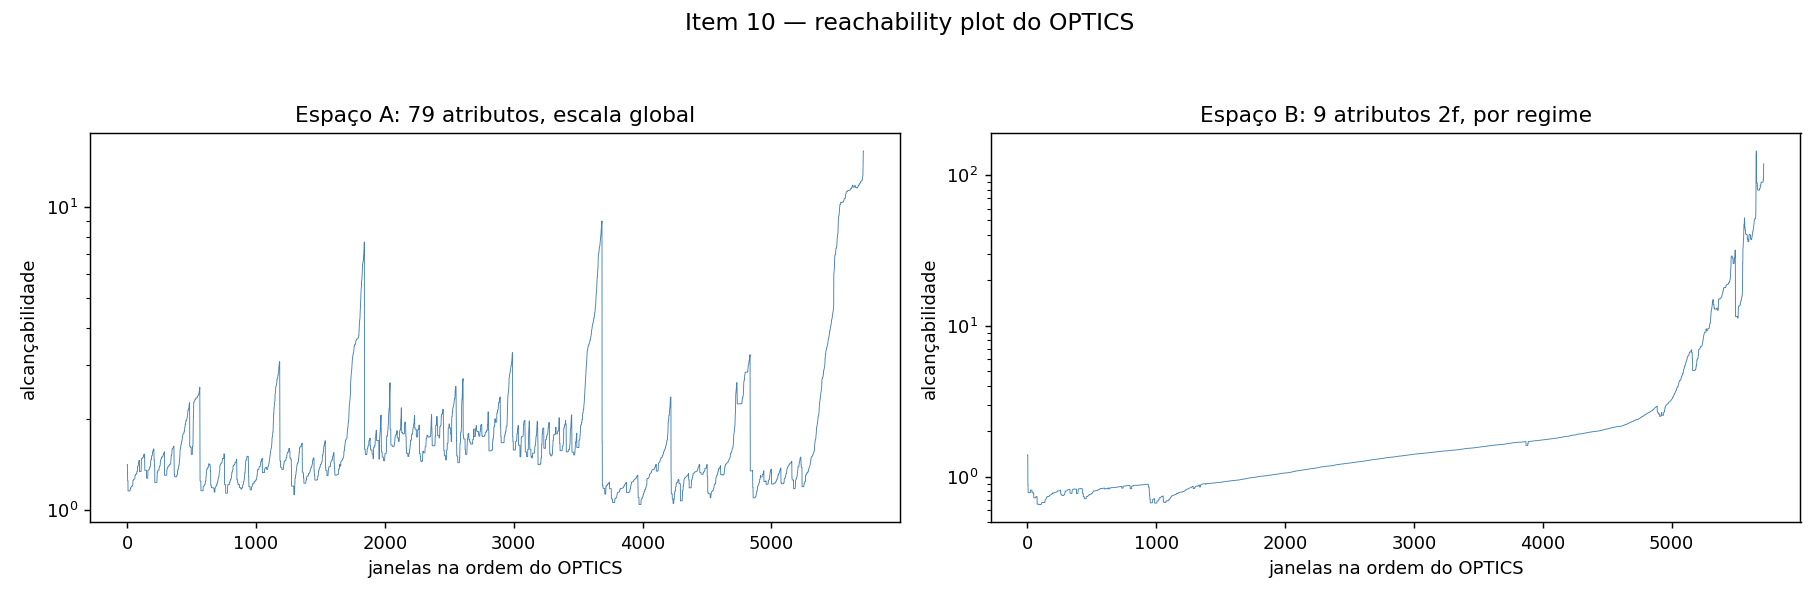
\includegraphics[width=\textwidth]{Figuras_Aula4/fig9-reachability-optics.png}
    \caption{\emph{Reachability plot} do OPTICS nos dois espaços, escala vertical logarítmica.}
    \label{fig:fig9}
\end{figure}

\subsection{Item 11 --- Métricas internas de todos os algoritmos}

\begin{table}[H]
\centering
\caption{Métricas internas dos doze algoritmos, nos dois espaços, com $K = 3$}
\label{tab:internas}
\begin{tabular}{llccccc}
\toprule
Espaço & Algoritmo & Grupos & Ruído (\%) & Silhueta & Calinski-H. & Davies-B. \\
\midrule
A & K-Means                 & 3  & 0{,}0  & 0{,}329 & 2387 & 1{,}079 \\
A & MiniBatch K-Means       & 3  & 0{,}0  & 0{,}329 & 2387 & 1{,}079 \\
A & Aglomerativo (Ward)     & 3  & 0{,}0  & 0{,}322 & 2314 & 1{,}084 \\
A & Aglomerativo (Complete) & 3  & 0{,}0  & 0{,}588 & 995  & 1{,}379 \\
A & DBSCAN                  & 11 & 12{,}7 & 0{,}231 & 1062 & 1{,}795 \\
A & GMM                     & 3  & 0{,}0  & 0{,}283 & 1447 & 1{,}648 \\
A & Spectral                & 3  & 0{,}0  & 0{,}287 & 367  & 1{,}749 \\
A & Mean Shift              & 51 & 0{,}0  & 0{,}271 & 48   & 0{,}658 \\
A & BIRCH                   & 3  & 0{,}0  & 0{,}321 & 2310 & 1{,}082 \\
A & Affinity Propagation    & 79 & 0{,}0  & 0{,}265 & 201  & 1{,}106 \\
A & HDBSCAN                 & 3  & 5{,}2  & 0{,}349 & 2325 & 1{,}611 \\
A & OPTICS                  & 20 & 58{,}5 & 0{,}387 & 670  & 0{,}889 \\
\midrule
B & K-Means                 & 3   & 0{,}0  & 0{,}925 & 28961 & 0{,}376 \\
B & MiniBatch K-Means       & 3   & 0{,}0  & 0{,}828 & 11993 & 0{,}693 \\
B & Aglomerativo (Ward)     & 3   & 0{,}0  & 0{,}931 & 26506 & 0{,}317 \\
B & Aglomerativo (Complete) & 3   & 0{,}0  & 0{,}931 & 28275 & 0{,}329 \\
B & DBSCAN                  & 2   & 14{,}2 & 0{,}595 & 624   & 0{,}477 \\
B & GMM                     & 3   & 0{,}0  & 0{,}793 & 13192 & 0{,}749 \\
B & Spectral                & 3   & 0{,}0  & 0{,}772 & 2272  & 0{,}785 \\
B & Mean Shift              & 50  & 0{,}0  & 0{,}754 & 3610  & 0{,}311 \\
B & BIRCH                   & 3   & 0{,}0  & 0{,}931 & 26506 & 0{,}317 \\
B & Affinity Propagation    & 173 & 0{,}0  & 0{,}129 & 15345 & 0{,}604 \\
B & HDBSCAN                 & 2   & 4{,}0  & 0{,}900 & 4198  & 0{,}168 \\
B & OPTICS                  & 3   & 5{,}8  & \textbf{0{,}931} & \textbf{80151} & \textbf{0{,}163} \\
\bottomrule
\end{tabular}
\end{table}

\noindent \textbf{Ressalva obrigatória.} Para DBSCAN, HDBSCAN e OPTICS as três métricas foram calculadas \textbf{apenas sobre os pontos não-ruidosos}. O OPTICS lidera as três no espaço B descartando 5,8\% dos pontos, e no espaço A o mesmo OPTICS aparece com a melhor silhueta descartando \textbf{58,5\%}. A coluna de ruído tem de ser lida junto com as demais.

\subsection{Item 12 --- Métricas externas para os dois rótulos}

\begin{table}[H]
\centering
\caption{Métricas externas contra o rótulo \textbf{condição} (3 classes; taxa base 0,773)}
\label{tab:externas-condicao}
\begin{tabular}{llcccc}
\toprule
Espaço & Algoritmo & ARI & NMI & V-measure & Pureza \\
\midrule
B & DBSCAN                  & \textbf{0{,}592} & 0{,}389 & 0{,}389 & 0{,}851 \\
B & GMM                     & 0{,}530 & 0{,}375 & 0{,}375 & 0{,}850 \\
B & Spectral                & 0{,}516 & \textbf{0{,}397} & \textbf{0{,}397} & 0{,}839 \\
B & MiniBatch K-Means       & 0{,}489 & 0{,}388 & 0{,}388 & 0{,}852 \\
B & OPTICS                  & 0{,}360 & 0{,}285 & 0{,}285 & 0{,}831 \\
B & Mean Shift              & 0{,}342 & 0{,}276 & 0{,}276 & 0{,}828 \\
B & HDBSCAN                 & 0{,}255 & 0{,}231 & 0{,}231 & 0{,}819 \\
A & GMM                     & 0{,}228 & 0{,}262 & 0{,}262 & 0{,}854 \\
B & K-Means                 & 0{,}177 & 0{,}181 & 0{,}181 & 0{,}807 \\
A & Aglomerativo (Complete) & 0{,}167 & 0{,}171 & 0{,}171 & 0{,}805 \\
B & Aglomerativo (Complete) & 0{,}147 & 0{,}152 & 0{,}152 & 0{,}801 \\
B & Aglomerativo (Ward)     & 0{,}138 & 0{,}143 & 0{,}143 & 0{,}799 \\
B & BIRCH                   & 0{,}138 & 0{,}143 & 0{,}143 & 0{,}799 \\
A & K-Means                 & 0{,}075 & 0{,}102 & 0{,}102 & 0{,}805 \\
A & MiniBatch K-Means       & 0{,}075 & 0{,}102 & 0{,}102 & 0{,}805 \\
A & Mean Shift              & 0{,}071 & 0{,}116 & 0{,}116 & 0{,}808 \\
A & BIRCH                   & 0{,}065 & 0{,}103 & 0{,}103 & 0{,}805 \\
A & HDBSCAN                 & 0{,}065 & 0{,}117 & 0{,}117 & 0{,}822 \\
A & Aglomerativo (Ward)     & 0{,}064 & 0{,}103 & 0{,}103 & 0{,}805 \\
A & DBSCAN                  & 0{,}028 & 0{,}091 & 0{,}091 & 0{,}823 \\
B & Affinity Propagation    & 0{,}014 & 0{,}154 & 0{,}154 & \textbf{0{,}883} \\
A & Affinity Propagation    & 0{,}005 & 0{,}071 & 0{,}071 & 0{,}807 \\
A & Spectral                & $-0{,}001$ & 0{,}003 & 0{,}003 & 0{,}759 \\
A & OPTICS                  & $-0{,}082$ & 0{,}025 & 0{,}025 & 0{,}773 \\
\bottomrule
\end{tabular}
\end{table}

\begin{table}[H]
\centering
\caption{Métricas externas contra o rótulo \textbf{regime de operação} (9 classes; taxa base 0,111)}
\label{tab:externas-regime}
\begin{tabular}{llccccc}
\toprule
Espaço & Algoritmo & Grupos & ARI & NMI & V-measure & Pureza \\
\midrule
A & DBSCAN                  & 11 & \textbf{0{,}681} & \textbf{0{,}799} & \textbf{0{,}799} & 0{,}803 \\
A & Spectral                & 3  & 0{,}385 & 0{,}632 & 0{,}632 & 0{,}351 \\
A & HDBSCAN                 & 3  & 0{,}384 & 0{,}605 & 0{,}605 & 0{,}323 \\
A & Mean Shift              & 51 & 0{,}282 & 0{,}508 & 0{,}508 & 0{,}347 \\
A & Affinity Propagation    & 79 & 0{,}279 & 0{,}665 & 0{,}665 & \textbf{0{,}933} \\
A & OPTICS                  & 20 & 0{,}195 & 0{,}546 & 0{,}546 & 0{,}526 \\
A & K-Means                 & 3  & 0{,}179 & 0{,}417 & 0{,}417 & 0{,}219 \\
A & MiniBatch K-Means       & 3  & 0{,}179 & 0{,}417 & 0{,}417 & 0{,}219 \\
A & Aglomerativo (Ward)     & 3  & 0{,}169 & 0{,}389 & 0{,}389 & 0{,}216 \\
A & BIRCH                   & 3  & 0{,}169 & 0{,}389 & 0{,}389 & 0{,}216 \\
A & GMM                     & 3  & 0{,}167 & 0{,}366 & 0{,}366 & 0{,}213 \\
A & Aglomerativo (Complete) & 3  & 0{,}000 & 0{,}012 & 0{,}012 & 0{,}115 \\
\midrule
B & \emph{os doze algoritmos} & --- & $-0{,}000$ a $0{,}026$ & --- & --- & --- \\
\bottomrule
\end{tabular}
\end{table}

\noindent A última linha é uma \textbf{verificação de que a normalização funcionou}. No espaço B o ARI contra regime fica entre $-0{,}000$ e $0{,}026$ para os doze algoritmos: padronizar pelas janelas saudáveis do próprio regime \textbf{removeu} a informação de ponto de operação, que é exatamente o que se pretendia.

\subsubsection*{Três armadilhas de métrica que este conjunto expõe}

\textbf{Armadilha 1 --- a Pureza da condição gira em torno da taxa base.} A classe majoritária vale $4419/5715 = 0{,}773$, e quase todos os algoritmos entregam Pureza entre 0,80 e 0,85. Um leitor que olhasse só essa coluna concluiria que todos os métodos são equivalentes. O ARI, que corrige pelo acaso, mostra uma faixa de $-0{,}082$ a $0{,}592$.

\textbf{Armadilha 2 --- Pureza cresce trivialmente com o número de grupos.} O \emph{Affinity Propagation} tem a melhor Pureza das duas tabelas --- 0,883 contra condição e \textbf{0,933} contra regime --- e ARI de 0,014 e 0,279, com 173 e 79 grupos para 3 e 9 classes.

\textbf{Armadilha 3 --- métricas internas podem apontar o oposto das externas.} No espaço B, Ward e BIRCH atingem silhueta \textbf{0,931} e Calinski-Harabasz \textbf{26506} com ARI de apenas \textbf{0,138}. São partições geometricamente excelentes do objeto errado: dividem a massa saudável em vez de isolar as faltas. É o exemplo mais nítido produzido neste trabalho de que \textbf{métrica interna não substitui rótulo}.

\subsection{Item 13 --- Síntese comparativa e recomendação}

\begin{figure}[H]
    \centering
    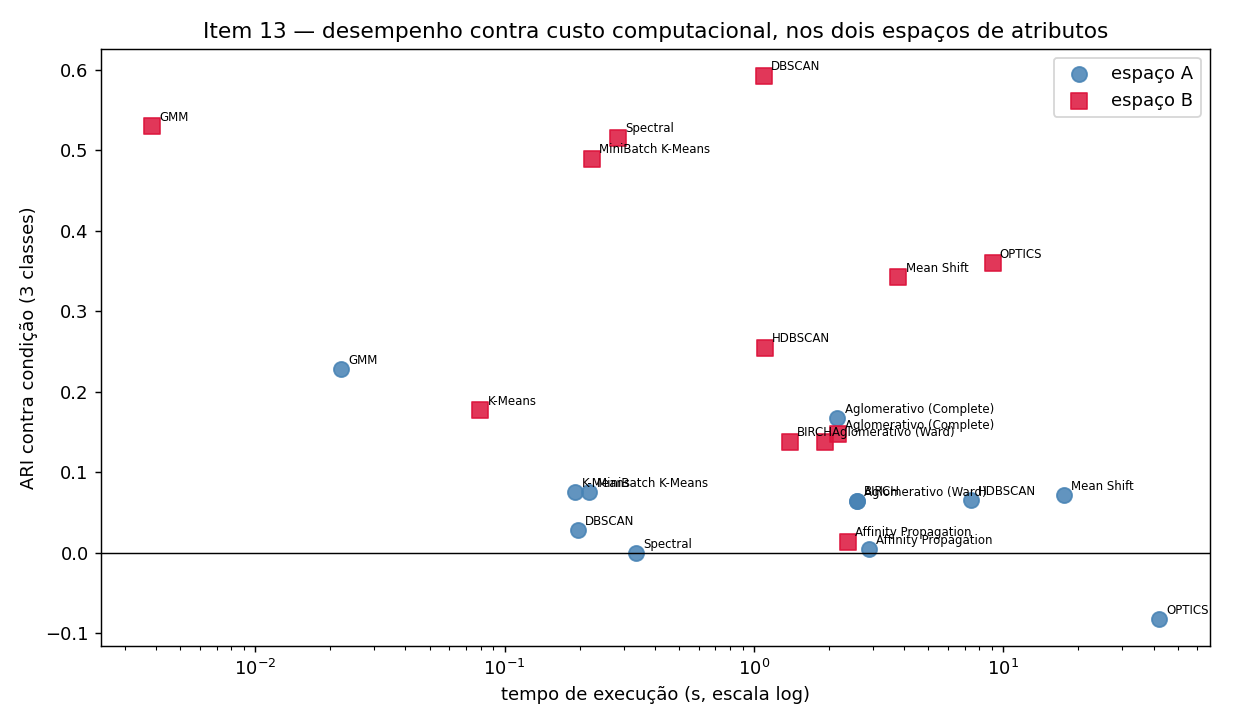
\includegraphics[width=0.95\textwidth]{Figuras_Aula4/fig10-desempenho-custo.png}
    \caption{Desempenho (ARI contra condição) \emph{versus} custo computacional, em escala logarítmica de tempo, nos dois espaços.}
    \label{fig:fig10}
\end{figure}

\begin{table}[H]
\centering
\caption{Síntese: desempenho, custo e interpretabilidade (os sete melhores)}
\label{tab:sintese}
\begin{tabular}{llccccl}
\toprule
Esp. & Algoritmo & ARI & Ruído & Prec.\ do & Tempo & Interpretabilidade \\
     &           & cond. & (\%) & ruído & (s) & \\
\midrule
B & DBSCAN            & \textbf{0{,}592} & 14{,}2 & \textbf{0{,}904} & 1{,}09 & Alta (densidade + ruído rotulável) \\
B & GMM               & 0{,}530 & 0{,}0  & ---     & 0{,}00 & Alta (densidades e probabilidades) \\
B & Spectral          & 0{,}516 & 0{,}0  & ---     & 0{,}28 & Baixa (\emph{embedding} espectral) \\
B & MiniBatch K-Means & 0{,}489 & 0{,}0  & ---     & 0{,}22 & Alta (centróides) \\
B & OPTICS            & 0{,}360 & 5{,}8  & \textbf{1{,}000} & 9{,}04 & Média (\emph{reachability}) \\
B & Mean Shift        & 0{,}342 & 0{,}0  & ---     & 3{,}79 & Média (modos) \\
B & HDBSCAN           & 0{,}255 & 4{,}0  & \textbf{1{,}000} & 1{,}11 & Média (hierarquia + ruído) \\
\bottomrule
\end{tabular}
\end{table}

\noindent \textbf{Os sete melhores são todos do espaço B.} O melhor resultado do espaço A --- GMM, ARI 0,228 --- fica abaixo do sétimo colocado do espaço B. \textbf{A escolha do espaço de atributos vale mais que a escolha do algoritmo}, e por uma margem grande.

\subsubsection*{Recomendação para monitoramento contínuo em produção}

\textbf{Algoritmo recomendado: DBSCAN sobre o espaço B.} A justificativa tem quatro pontos:

\begin{enumerate}[nosep]
    \item \textbf{Desempenho:} maior ARI contra condição entre todos (\textbf{0,592}), acima de GMM (0,530) e Spectral (0,516).
    \item \textbf{A saída é diretamente acionável:} o rótulo $-1$ \textbf{é} o alarme. Com precisão de 0,904 e 4,0 vezes a taxa base, o conjunto de ruído pode ser encaminhado para inspeção sem nenhum pós-processamento. Nenhum método sem ruído oferece isso.
    \item \textbf{Custo:} 1,09\,s para 5715 janelas, contra 17,5\,s do Mean Shift no espaço A.
    \item \textbf{Interpretabilidade:} decisão explicável por densidade local e por um limiar \texttt{eps} auditável, ao contrário do \emph{Spectral}.
\end{enumerate}

\textbf{Ressalva que acompanha a recomendação.} O DBSCAN \textbf{não é incremental}. Num monitoramento que recebe uma janela a cada 50\,ms, reajustar o modelo a cada lote é inviável. A arquitetura correta em produção é usar o DBSCAN \emph{offline} para \textbf{calibrar} o limiar sobre um histórico saudável e, em linha, aplicar apenas o indicador escalar de ondulação em $2f$ normalizado pelo regime --- operação de custo $O(1)$ por janela. Se for exigido um algoritmo que se atualize em linha, o BIRCH é incremental por construção, mas entrega ARI de 0,138 e não é recomendável para esta tarefa.

\textbf{Segunda ressalva.} A recomendação vale para \textbf{detectar} falta. Para \textbf{reconhecer o regime de operação} o espaço correto é o A, no qual o DBSCAN atinge ARI de 0,681 contra o rótulo de regime. São duas tarefas distintas que pedem espaços de atributos distintos, e a arquitetura em produção deveria manter os dois.

\newpage
% ============================================================
\section{Considerações Finais}

\begin{itemize}
    \item \textbf{A falta é detectável, e a assinatura é a ondulação em $2\omega$.} Um curto assimétrico gera sequência negativa, e sequência negativa aparece em $2\omega$ no referencial que gira a $+\omega$. Nove atributos construídos sobre esse princípio, num espaço de dimensão efetiva 2, entregam ARI de 0,592 contra as três classes de condição.

    \item \textbf{A escolha do espaço de atributos domina a escolha do algoritmo.} Os sete melhores resultados da Tabela~\ref{tab:sintese} são todos do espaço B. O \emph{Spectral Clustering} passa de pior método ($-0{,}001$) a terceiro melhor (0,516) sem que uma linha da sua configuração mude. Uma análise preliminar restrita a estatísticas temporais das correntes de fase concluiu que a falta era indetectável e atribuiu o fato à física do controle orientado por campo; o conjunto completo mostra que a limitação era dos atributos, não do sistema.

    \item \textbf{O ruído dos métodos de densidade não tem interpretação universal.} No espaço A ele mistura regimes e faltas; no espaço B ele é falta em 90,4\% dos casos, e HDBSCAN e OPTICS chegam a 100\% de precisão. A pergunta ``anomalia real ou baixa densidade?'' só se responde medindo a composição do ruído.

    \item \textbf{Métricas externas e internas exigem leitura crítica.} Este conjunto expõe três armadilhas de forma nítida: Pureza igual à taxa base, Pureza inflada por excesso de grupos, e silhueta de 0,931 acompanhada de ARI de 0,138.

    \item \textbf{Os critérios automáticos falharam duas vezes e foram corrigidos com justificativa.} O joelho da curva de $k$-distância superestima \texttt{eps} quando a cauda é longa, e a heurística $n/60$ para \texttt{min\_cluster\_size} do HDBSCAN cai numa transição abrupta que leva de 4\% a 94\% de ruído. Ambos foram substituídos por critérios verificados por varredura.

    \item \textbf{A silhueta discorda do número de classes reais, e isso é informação.} Ela aponta $K=2$ nos dois espaços quando existem 3 classes, porque 77,3\% das janelas são saudáveis. Em conjuntos desbalanceados o critério de silhueta mede separação, não correspondência com a semântica do problema.
\end{itemize}

\subsection*{Uma observação sobre o método de trabalho}

Os dois erros corrigidos ao longo deste estudo --- usar 3 de 35 canais e trabalhar com 21 de 225 ensaios --- têm a mesma forma: \textbf{uma limitação foi declarada sem ter sido verificada na fonte}. Nos dois casos a frase escrita era ``não é possível com estes dados'', e nos dois casos ela era falsa.

Isso importa para além deste exercício. Um resultado negativo bem argumentado é mais perigoso que um resultado negativo mal argumentado, porque ele encerra a investigação. O primeiro laudo deste trabalho tinha modelo nulo, controle positivo, análise de poder e uma explicação física coerente --- e ainda assim estava errado, porque toda essa estrutura foi aplicada sobre um recorte que nunca foi justificado.

A salvaguarda que funcionou não foi estatística. Foi perguntar, duas vezes, \emph{o que foi deixado de fora?}

% ============================================================
\section*{Apêndice: validação estatística}
\addcontentsline{toc}{section}{Apêndice: validação estatística}

A assinatura em $2f$ foi validada \textbf{antes} de qualquer agrupamento, por três vias independentes, com hipótese física declarada previamente.

\subsection*{Modelos nulos}

Dois nulos independentes, ambos preservando a estrutura temporal do registro:
\begin{enumerate}[nosep]
    \item \textbf{N1} --- mesmo contraste de intervalos aplicado aos ensaios \texttt{HEALTHY}, nos quais o contator nunca fecha.
    \item \textbf{N2} --- contraste entre dois sub-intervalos \emph{dentro} do trecho saudável dos próprios ensaios com falta: mesmo arquivo, mesmo regime, mesma sessão.
\end{enumerate}

\noindent O teste é de \textbf{excedência}: sob o nulo, cada ensaio excede o percentil 95 com probabilidade 0,05, de modo que observar $k$ de $n$ excedências tem $p$ binomial exato. Os nove atributos de ondulação em $2f$ passam \textbf{nos dois nulos} com correção de Bonferroni para 79 atributos, com $p$ entre $10^{-8}$ e $10^{-12}$.

\subsection*{Sensibilidade e falso alarme, por regime}

\begin{table}[H]
\centering
\caption{Excedências do nulo do próprio regime, por ponto de operação}
\begin{tabular}{lcc}
\toprule
Regime & Falta entre enrolamentos & Falta entre espiras \\
\midrule
S1200 (três torques) & 10--11 / 12 & 8 / 12 \\
S1500 (três torques) & 7--9 / 12   & \textbf{2--5 / 12} \\
S1800 (três torques) & \textbf{12 / 12} & 9 / 12 \\
\midrule
\textbf{Total} & \textbf{91/108 (84\%)} & \textbf{61/108 (56\%)} \\
               & $p = 4{,}7\times10^{-100}$ & $p = 4{,}1\times10^{-50}$ \\
\bottomrule
\end{tabular}
\end{table}

\noindent A assinatura vale nos nove pontos de operação, mas não uniformemente. O pior é o \textbf{S1500}, que é o mesmo ponto de operação que os métodos de densidade tratam como atípico em todas as análises --- a bancada tem comportamento distinto ali.

\textbf{Falso alarme cross-regime:} no limiar do percentil 99 das janelas saudáveis, apenas \textbf{6 alarmes em 531 janelas} saudáveis, distribuídos entre 0 e 2 por regime. O indicador normalizado por regime está calibrado e \textbf{não deriva} quando o ponto de operação muda.

\subsection*{Falseador: o sinal tem de voltar quando o contator abre}

\begin{figure}[H]
    \centering
    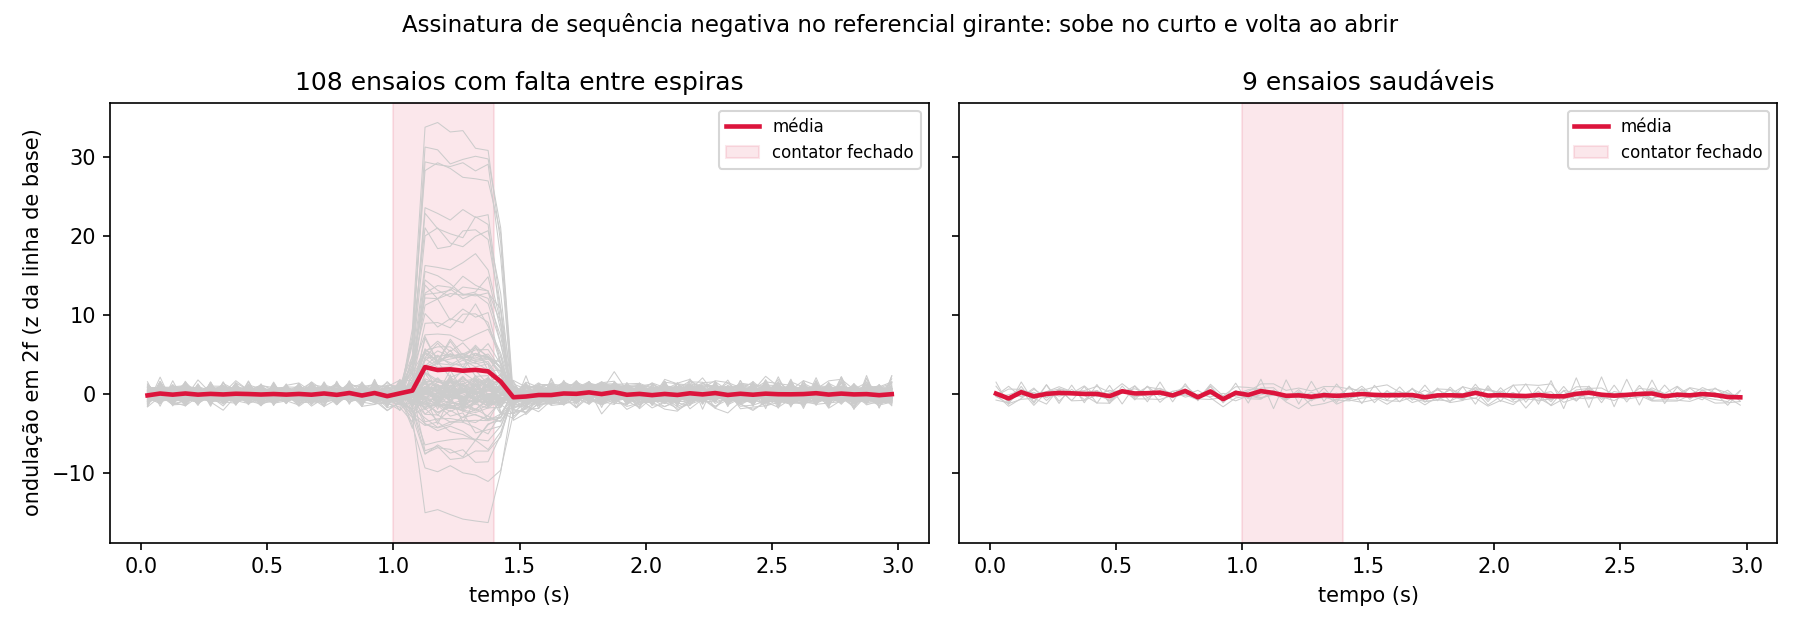
\includegraphics[width=0.95\textwidth]{Figuras_Aula4/fig12-ondulacao-2f-recuperacao.png}
    \caption{Indicador composto de ondulação em $2f$ ao longo dos 3\,s, padronizado pela linha de base de cada ensaio. Faixa sombreada: contator fechado.}
    \label{fig:fig12}
\end{figure}

\noindent Nos 108 ensaios com falta entre espiras o indicador vai a $\mathbf{+2{,}68\sigma}$ durante o curto e retorna a $\mathbf{-0{,}03\sigma}$ depois que o contator abre. Nos 9 ensaios saudáveis permanece plano. Deriva lenta do ensaio subiria e não voltaria; o padrão observado é de resposta a evento.

Adotando como limiar o maior pico observado \emph{fora} do curto nos ensaios saudáveis, \textbf{62 dos 108 ensaios} são detectados com \textbf{zero falsos positivos}.

\begin{figure}[H]
    \centering
    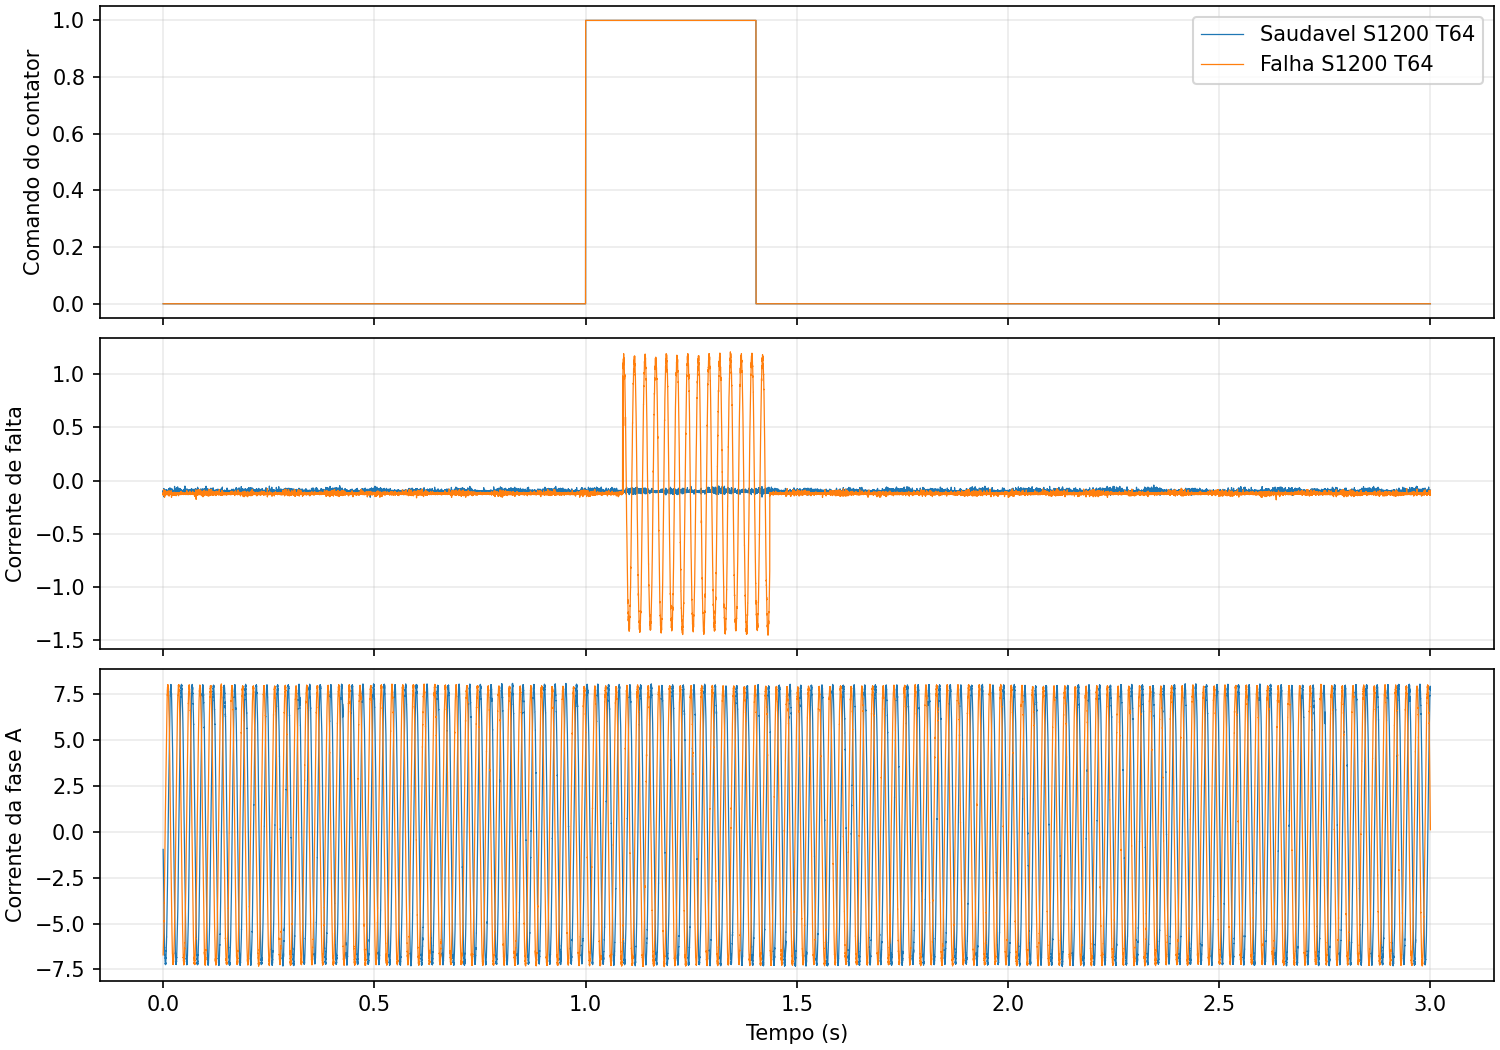
\includegraphics[width=0.85\textwidth]{Figuras_Aula4/fig11-corrente-falta-sequencia-negativa.png}
    \caption{Comando do contator, corrente de falta e corrente de fase, para ensaio saudável e ensaio com falta no mesmo ponto de operação.}
    \label{fig:fig11}
\end{figure}

\subsection*{Dose-resposta e decomposição severidade $\times$ posição}

A magnitude do indicador escala com a corrente de falta medida: \textbf{Spearman $\rho = 0{,}738$}, $p = 8{,}8\times10^{-20}$, $n = 108$. O indicador não apenas acende --- ele mede.

Quanto à decomposição, a severidade entra primeiro porque o par de derivação \textbf{carrega} a severidade:
\begin{itemize}[nosep]
    \item $\text{AUC} \sim \log(I_{\text{falta}})$ dá $R^2 = 0{,}415$: a severidade sozinha explica 41\%.
    \item Do resíduo estruturado, o par responde por 65\% e o regime por 35\%.
\end{itemize}
\noindent A leitura defensável é \textbf{severidade primeiro, posição como efeito secundário não descartável}. Separar de vez exigiria ensaios com resistências de falta diferentes no mesmo par, que não existem neste dataset.

\subsection*{Poder do teste}

Degraus sintéticos de amplitude conhecida injetados nos ensaios saudáveis mostram que o teste de recuperação detecta efeitos de \textbf{2 a 4 desvios robustos} nos melhores canais. O controle positivo, usando a própria corrente de falta como atributo, produz efeito de 2191 desvios contra percentil 95 do nulo de 0,59. O poder não é o fator limitante.

\subsection*{Correção do ângulo elétrico}

O script de exemplo distribuído pelos autores utiliza \texttt{2*Theta\_est - pi/2}. A medição mostra que isso é incorreto para este dataset: com \texttt{Theta\_est} o eixo direto fica praticamente constante (desvio 0,15 contra média 4,08), enquanto com \texttt{2*Theta\_est - pi/2} ele oscila na fundamental. Portanto \texttt{Theta\_est} \textbf{já é} o ângulo elétrico; o fator 2 provavelmente foi herdado do dataset PMSG dos mesmos autores, no qual o ângulo medido é mecânico.

\subsection*{Reprodutibilidade}

Semente fixa \texttt{20260923} em todos os algoritmos estocásticos. Algoritmos de custo $O(n^2)$ --- \emph{Spectral}, \emph{Mean Shift} e \emph{Affinity Propagation} --- foram avaliados em subamostra aleatória de 1500 janelas, o que está registrado nas tabelas de resultados.

Toda a cadeia está no notebook anexo, \texttt{Exercicio\_Aula4\_SCIG.ipynb}, que \textbf{executa integralmente e sem dependência de nenhum outro arquivo}: ele baixa os 225 ensaios do repositório oficial, verifica cada \texttt{.mat} antes de aceitá-lo, audita os 35 canais, extrai os 79 atributos, aplica os doze algoritmos nos dois espaços e gera as doze figuras e as tabelas deste relatório. São 49 células, 22 delas de código.

Duas notas de operação. A primeira célula de dados \textbf{só baixa o que faltar}: se os 225 ensaios já estiverem em disco, ela apenas confere o inventário. A célula de extração grava \texttt{atributos\_completo.csv} e, em execuções seguintes, carrega esse arquivo em vez de reprocessar os 1,2\,GB de sinal bruto --- o que torna o notebook barato de reexecutar sem deixar de ser completo a partir do zero.

\end{document}
